%%%%%%%%%%%%%%%%%%%%%%%%%%%%%%%%%%%%
% This is the template for submission to ISCA 2018
% The cls file is a modified from  'sig-alternate.cls'
%%%%%%%%%%%%%%%%%%%%%%%%%%%%%%%%%%%%

\documentclass{sig-alternate} 
\usepackage{mathptmx} % This is Times font

\newcommand{\ignore}[1]{}
\usepackage{fancyhdr}
\usepackage[normalem]{ulem}
\usepackage[hyphens]{url}
\usepackage{microtype}

% Always include hyperref last
\usepackage[bookmarks=true,breaklinks=true,letterpaper=true,colorlinks,linkcolor=black,citecolor=blue,urlcolor=black]{hyperref}

% Ensure letter paper
\pdfpagewidth=8.5in
\pdfpageheight=11in


%%%%%%%%%%%---SETME-----%%%%%%%%%%%%%
\newcommand{\iscasubmissionnumber}{380}
%%%%%%%%%%%%%%%%%%%%%%%%%%%%%%%%%%%%

\fancypagestyle{firstpage}{
  \fancyhf{}
\setlength{\headheight}{50pt}
\renewcommand{\headrulewidth}{0pt}
  \fancyhead[C]{\normalsize{ISCA 2018 Submission
      \textbf{\#\iscasubmissionnumber} \\ Confidential Draft: DO NOT DISTRIBUTE}} 
  \pagenumbering{arabic}
}

\usepackage{amsmath,amsfonts,amssymb}
\usepackage{graphicx}
\usepackage{subfigure}
\usepackage{algorithm}
\usepackage{algorithmicx}
\usepackage{algpseudocode}
\usepackage{caption}
\usepackage{multirow}
\usepackage{textcomp,booktabs}
\usepackage[usenames,dvipsnames]{color}
\usepackage{colortbl}
\usepackage{indentfirst}
\usepackage{url}
\usepackage{cite}
% \usepackage{bibspacing}
\usepackage{threeparttable}
\usepackage{bigstrut}


\usepackage{blindtext, graphicx}
\usepackage{epsfig}
\usepackage{syntonly}
\usepackage{rotating}
\usepackage{amsmath}
\usepackage{setspace}
\usepackage{verbatim} 
\usepackage{amssymb}
\usepackage{amsmath}
\setcounter{tocdepth}{3}
\usepackage{graphicx}
\usepackage{multirow}
\usepackage{colortbl}
\usepackage{enumerate}
\usepackage{color}
\usepackage{wrapfig}

%\usepackage[noend]{algorithm2e}
\usepackage{cleveref}
\usepackage{comment}
\usepackage{ifthen}
\usepackage[dotinlabels]{titletoc}
\usepackage{colortbl}
\usepackage{array}
\usepackage{alltt}
\usepackage{bm}
\renewcommand{\ttdefault}{txtt}
\usepackage[normalem]{ulem}


% \usepackage{mathptmx} % This is Times font
\pdfoutput=1 %for posting to arXiv
\usepackage{blindtext, graphicx}
\usepackage{epsfig}
\usepackage{syntonly}
\usepackage{rotating}
\usepackage{amsmath}
\usepackage{setspace}
\usepackage{verbatim} 
\usepackage{amssymb}
\usepackage{amsmath}
\setcounter{tocdepth}{3}
\usepackage{graphicx}
\usepackage{multirow}
\usepackage{colortbl}
\usepackage{enumerate}
\usepackage{color}
\usepackage{wrapfig}
\usepackage{cleveref}
\usepackage{comment}
\usepackage{ifthen}
\usepackage[dotinlabels]{titletoc}
\usepackage{colortbl}
\usepackage{array}

\usepackage{alltt}
\usepackage{bm}
\usepackage{longtable,booktabs}
\usepackage{url}
\usepackage{courier}
\usepackage{cite}


\usepackage{tabularx}
\usepackage{footnote}

\newcommand{\SH}[1]{{\color{blue}{}\textbf{}{}}}
\newcommand{\YW}[1]{{\color{blue}{}\textbf{}{}}}

% \newcommand{\SH}[1]{{\color{blue}{[}\textbf{SH: #1}{]}}}
% \newcommand{\YH}[1]{{\color{blue}{[}\textbf{YW: #1}{]}}}





\usepackage{colortbl}
%\usepackage[justification=centering]{caption}
\usepackage{threeparttable}
\usepackage[free-standing-units]{siunitx}

\usepackage{listings}
\usepackage[usenames,dvipsnames]{xcolor}
\lstset{
language=C++,
basicstyle=\small,
numbers=left,
columns=flexible,
numbersep=5pt,
breaklines=true,
escapeinside= ``,
xleftmargin=20pt,
frame=tb,
framexleftmargin=20pt
}
\newcommand{\rev}[1]{\textcolor{blue}{{}#1}}
\renewcommand*\thelstnumber{\arabic{lstnumber}:}
\DeclareCaptionFormat{mylst}{\hrule#1#2#3}
\captionsetup[lstlisting]{format=mylst,labelfont=bf,singlelinecheck=off,labelsep=space}

%%%%%%%%%%%---SETME-----%%%%%%%%%%%%%
\title{Efficient Training Engine for Convolutional Neural Network with Structured Sparsity} 
\author{}
%%%%%%%%%%%%%%%%%%%%%%%%%%%%%%%%%%%%

\begin{document}
\maketitle
\thispagestyle{firstpage}
\pagestyle{plain}

\begin{abstract}

Training convolutional neural network (CNN) usually requires large amount of computation resource, time and power. Researchers and cloud service providers in this region needs fast and efficient training system. GPU is currently the best candidate for CNN training. But FPGAs have already shown good performance and energy efficiency as CNN inference accelerators. In this work, we design a compressed training process together with an FPGA-based accelerator for energy efficient CNN training. We adopt two of the widely used model compression methods, quantization and pruning, to accelerate CNN training process. 

The difference between inference and training brought challenges to apply the two methods in training. First, training requires higher data precision. We use the gradient accumulation buffer to achieve low operation complexity while keeping gradient descent precision. Second, sparse network results in different types of functions in forward and back-propagation phases. We design a novel architecture to utilize both inference and back-propagation sparsity. Experimental results show that the proposed training process achieves similar accuracy compared with traditional training process with floating point data. The proposed accelerator achieves 641GOP/s equivalent performance and 2.63x better energy efficiency compared with GPU. 

\end{abstract}

\section{Introduction}\label{sec:introduction}

% Deep neural networks (DNN) led to significant performance improvement in various AI applications, such as speech recognition \cite{RN164,RN165,RN167}, natural language processing \cite{RN168,Luong2015Effective,Wu2016Google}, reinforcement learning \cite{Mnih2013Playing, Mnih2015Human, Silver2016Mastering}, and computer vision (CV). Especially in computer vision, neural networks with convolution as a primary operation, named Convolutional Neural Network (CNN), become the most popular research methods \cite{He2016Deep, RN72,Redmon2016You, Shelhamer2017Fully, Simonyan2014Very}.

% Compared with traditional CV algorithms, neural network algorithms achieve superior performance benefited from the use of larger and deeper models and massive amount of training data~\cite{szegedy2015going, Simonyan2014Very, He2016Deep}. 
Convolutional neural networks (CNN) has made significant performance improvement in computer vision tasks \cite{He2016Deep, Shelhamer2017Fully}. However, the accuracy improvement comes at significant cost of training computation. 
% More and more researchers begin to focus on building efficient models to achieve the best accuracy with a limited model size. 

% In the study of reducing the computational complexity of neural networks, 
Model pruning and quantization have proved to be effective to reduce the requirements of computation, bandwidth and memory footprint, and have almost no effect on the performance (accuracy metric) of neural networks \cite{RN173,RN159,han2015deep}. A series of the hardware accelerator architecture designs are focused on the forward inference phase of neural networks, which takes full advantage of the benefits of sparseness and quantization and shows outstanding performance and energy efficiency. To deploy a sparse network, first the neural network model well-trained in dense needs to be pruned, and the loss of accuracy can be recovered by fine-tuning. Sparse neural networks can be deployed on different platforms and can achieve higher speed and energy efficiency than dense neural networks, as shown in Figure\ref{fig:intro}.

\begin{figure}[htbp]
  \centering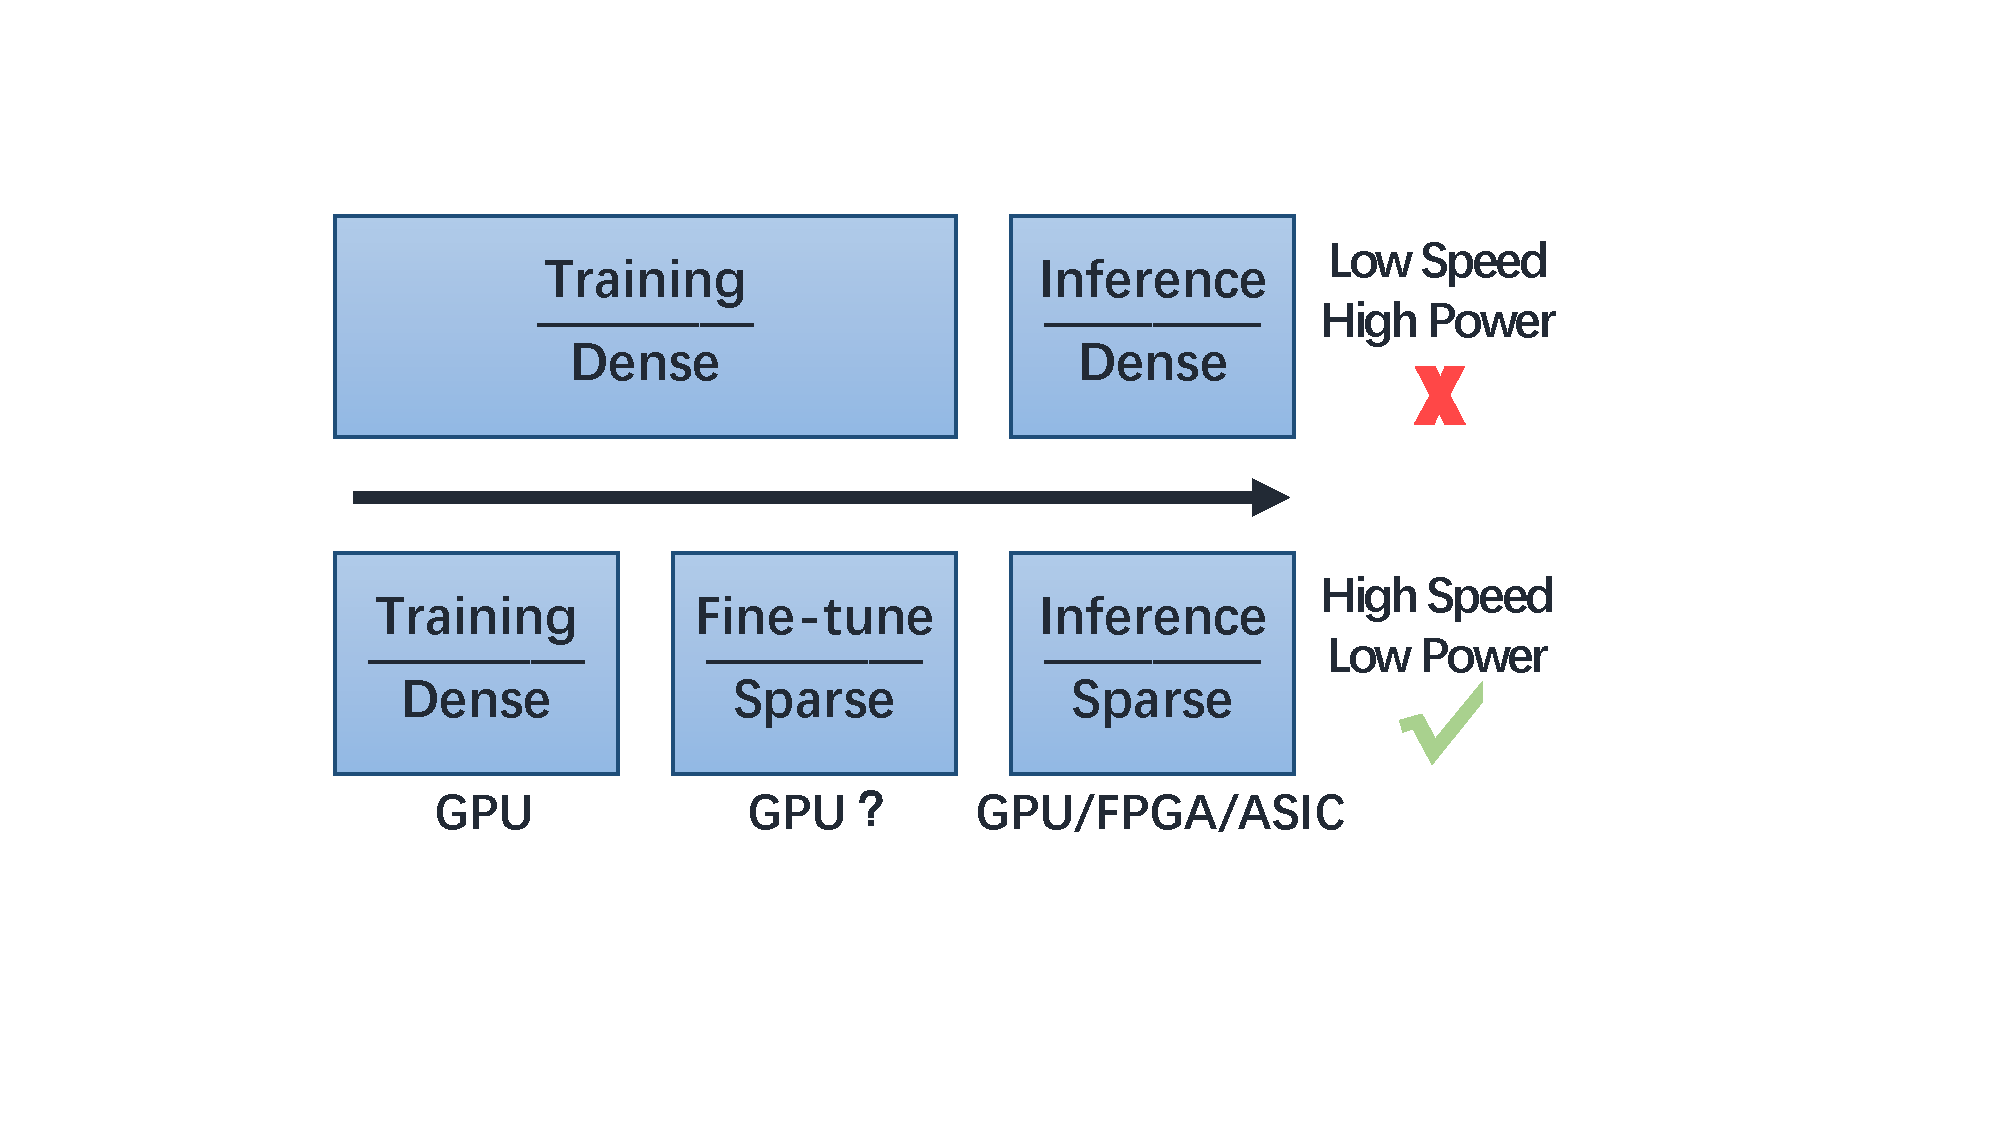
\includegraphics[width=3in]{figures/intro.pdf}
  \caption{Dense training, Sparse fine-tune, Sparse inference}\label{fig:intro}
\end{figure}

Although the GPU is suitable for training of dense neural networks, it can not be a proper user of the sparsity in the sparse neural network to further improve the performance (speed metric). Customized design hardware can make better use of the sparsity of the network to achieve the purpose of improving training efficiency. As a hardware programmable devices, FPGA has been widely deployed in the server cluster \cite{RN169, RN171, RN172}, but there is still no training architecture can take advantage of sparsity. On the other hand, the current fixed-point neural network training algorithm is still not hardware-friendly, for example, need floating point number to calculate the gradients\cite{Zhou2016DoReFa}.

In this paper, we propose an architecture design for sparse neural network training accelerators on the FPGA platform, which reached a high computing capability and energy efficiency. At the same time, we provide a sparse convolution neural network transformation technology, making the sparse neural network more suitable for training and inference on customized hardware platform while maintaining the accuracy at almost the same level. The main contributions of this paper are summarized as follows:
\begin{itemize}
\item A hardware friendly training process is proposed with all-fixed-point operations. 
\item Dedicated processing element (PE) on FPGA is designed to utilize the sparsity in both feed forward and back propagation phases of training.
\item We analyze the limitation on unroll parameters brought by sparsity and loop dimension variety between feed forward and back propagation phases. A corresponding flexible PE array structure is proposed to improve hardware utilization ratio.
\item Data arrangement and schedule strategies are proposed to improve bandwidth utilization .
\end{itemize}
Experimental results show that Proposed hardware achieves 641GOP/s equivalent performance and 3x better energy efficiency compared with GPU. 

The rest of this paper is organized as follows. Section~\ref{sec:preliminary} introduces the background of training of a CNN. Section~\ref{sec:related_work} reviews previous work on software and hardware level CNN optimization. Section~\ref{sec:training} and section~\ref{sec:hw} introduces the proposed training process and hardware platform respectively. Experimental results are shown in section~\ref{sec:experiment}. Section~\ref{sec:conclusion} concludes this paper.


\section{Preliminary}\label{sec:preliminary}

\subsection{Training Process of CNN}
Training of neural network is usually done with stochastic gradient descent. The training process consists of two alternate phases: forward(F) and back-propagation(BP). The forward phase randomly select a batch of training inputs and calculates their inference result with the current model. The backward phase first calculates the error between the inference result and the supervise data of corresponding inputs. Then the error is back-propagated through the network to calculate the gradient of the error to the weights.  

Training of CNN consists of two phases: feed forward (FF) and back propagation. Back propagation phase also consists two steps: calculating neuron gradients (NG) and weight gradients (WG). In this section, we introduce the computation of these three phases for training CNN.\Cref{tab:Notations} summarizes the symbols we use to explain CNN.

\begin{table}[htbp]
    \centering
    \caption{Notations to Explain CNN}
	\begin{tabular}{|l|p{5cm}|}
      \hline
      symbol & description \bigstrut\\
      \hline
      $d ^l$ & The output feature maps of $l^{th}$ layer \bigstrut\\
      \hline
      $\delta ^{l}$ & The error matrix of $l^{th}$ layer \bigstrut\\
      \hline
      $W ^{l}$,$\Delta W^{l}$ & The weights of of $l^{th}$ layer and its gradient. \bigstrut\\
      \hline
      $b ^ l$,$\Delta b ^ l$ & The bias of $l^{th}$ layer and its gradient \bigstrut\\
      \hline
      $ R^l$, $C^l $ & The row and column size of $d ^l$ \bigstrut\\
      \hline
      $ M^l$, $N^l $ & The input and output channel number of $l^{th}$ layer \bigstrut\\
      \hline
      $ K^l $ & The shape of a conv kernel is $K \times K$ \bigstrut\\
      \hline
    \end{tabular}%
    
    \label{tab:Notations}%
  \end{table}%
  
There are three kinds of layers in a typical CNN, \textit{convolutional(CONV) layer, Pooling layer, and fully connected(FC) layer}. Typically convolutional layers process 2-dimensional convolution to extract features. Pooling layers sub-sample the results of CONV layers to reduce the computation time and produce high-level features. The last few layers of a CNN are usually fully connected (FC) layers. FC layers convert the input 3-dimensional feature maps into a long 1-dimensional vector and do Matrix-Vector multiplication to produce output results.
  
\subsubsection{CONV layers}
In feed forward pass, CONV layers calculate 2-D convolution and sum the results of all input channels to produce one output channel. The pseudo code of a convolutional layer can be written as that in Listing \ref{code:conv_forward}.
  
\begin{minipage}{\linewidth}
\begin{lstlisting}[caption=Conv Forward, label=code:conv_forward]  
  for ( row=0; row<`$R^l$`; row++) { 
    for ( col=0; col<`$C^l$`; col++) { 
      for ( to=0; to<`$M^l$`; to++) { 
        `$d^l$`[to][row][col] = `$b^l$`[to];
        for ( ti =0; ti<`$N^l$`; ti++) { 
          for ( i =0; i<`$K^l$`; i++) { 
            for ( j=0; j<`$K^l$`; j++) {
              `$d^l$`[to][row][col] += \
                `$W^l$`[to][ti][i][j] * `$d^{l-1}$`[ti][row+i][col+j];
  } } } } } }

\end{lstlisting}
\end{minipage}

In back propagation pass, $\delta ^{l-1} , \Delta b^l, \Delta W^l$ will be calculated. The pseudo code of a convolutional layer can be written as that in Listing \ref{code:conv_back}. In each loop, the first multiplication accumulation (MAC) operation is in NG step and the second one is in WG step.
    
\begin{minipage}{\linewidth}
\begin{lstlisting}[caption=Conv Back propagation, label=code:conv_back]  
  for ( row=0; row<`$R^{l-1}$`; row++) { 
    for ( col=0; col<`$C^{l-1}$`; col++) { 
      for ( to=0; to<`$M^l$`; to++) { 
        `$\Delta b^{l}$`[to] += `$ \delta ^ l $`[to];
        for ( ti =0; ti<`$N^l$`; ti++) { 
          for ( i =0; i<`$K^l$`; i++) { 
            for ( j=0; j<`$K^l$`; j++) {
              `$\delta ^ {l-1}$`[ti][row][col] += \
                `$W^l$`[to][ti][i][j] * `$\delta ^ {l}$`[to][row-i][col-j] ;
              `$\Delta W^l$`[to][ti][i][j] += \
                `$\delta ^l$`[to][row-i][col-j] * `$d ^ {l-1} $`[ti][row][col];
  } } } } } }

\end{lstlisting}
\end{minipage}

\subsubsection{FC layers} \label{sec:prelim:fc}

All the elements in the input feature or output feature can be considered in a vector. The length of the input vector is $M$, and the output vector length is $N$. The forward process can be described in Listing \ref{code:fc_forward}.

\begin{minipage}{\linewidth}
\begin{lstlisting}[
  caption=FC Forward,
  label=code:fc_forward]
  for ( to=0; to<`$M$`; to++ ) {
    `$d^l$`[to] += `$b^l$`[to];
    for ( ti =0; ti<`$N$`; ti++) {
      `$d^l$`[to] += `$d^{l-1}$`[ti] * `$W$`[to][ti];
} }
\end{lstlisting}
\end{minipage}

As same as CONV layers,  $\delta ^{l-1} , \Delta b^l, \Delta W^l$ will be calculated in back propagation pass. The back propagation of FC layer is shown in Listing \ref{code:fc_backpropagation}.

\begin{minipage}{\linewidth}
\begin{lstlisting}[
  caption=FC Back propagation,
  label=code:fc_backpropagation]
for ( ti =0; ti<N; ti++ ){
  `$\Delta b^l$`[ti] = `$\delta ^ l$`[ti];
  for ( to=0; to<M; to++ ) {
    `$\delta ^ {l-1}$`[ti] += `$W$`[to][ti] * `$\delta ^ l$`[to];     
    `$\Delta W ^ l$`[ti][to] = `$d^{l-1}$`[ti]*`$\delta ^ l$`[to];
} }
\end{lstlisting}
\end{minipage}

\subsubsection{Pooling layers}
In FF phase, pooling layers down samples each channel of the input feature map. There are no weights for Pooling layers to train. A typical down sampling function is the max pooling function, which is to find the maximum value of small windows of the input feature maps. No WG step is needed for pooling layer. For NG step, a pooling layer upsamples the error according to the downsampling function. \Cref{fig:pool} illustrates an example of FF and NG step of a $2\times 2$ max pooling layer.
\begin{figure}[htbp]
    \centering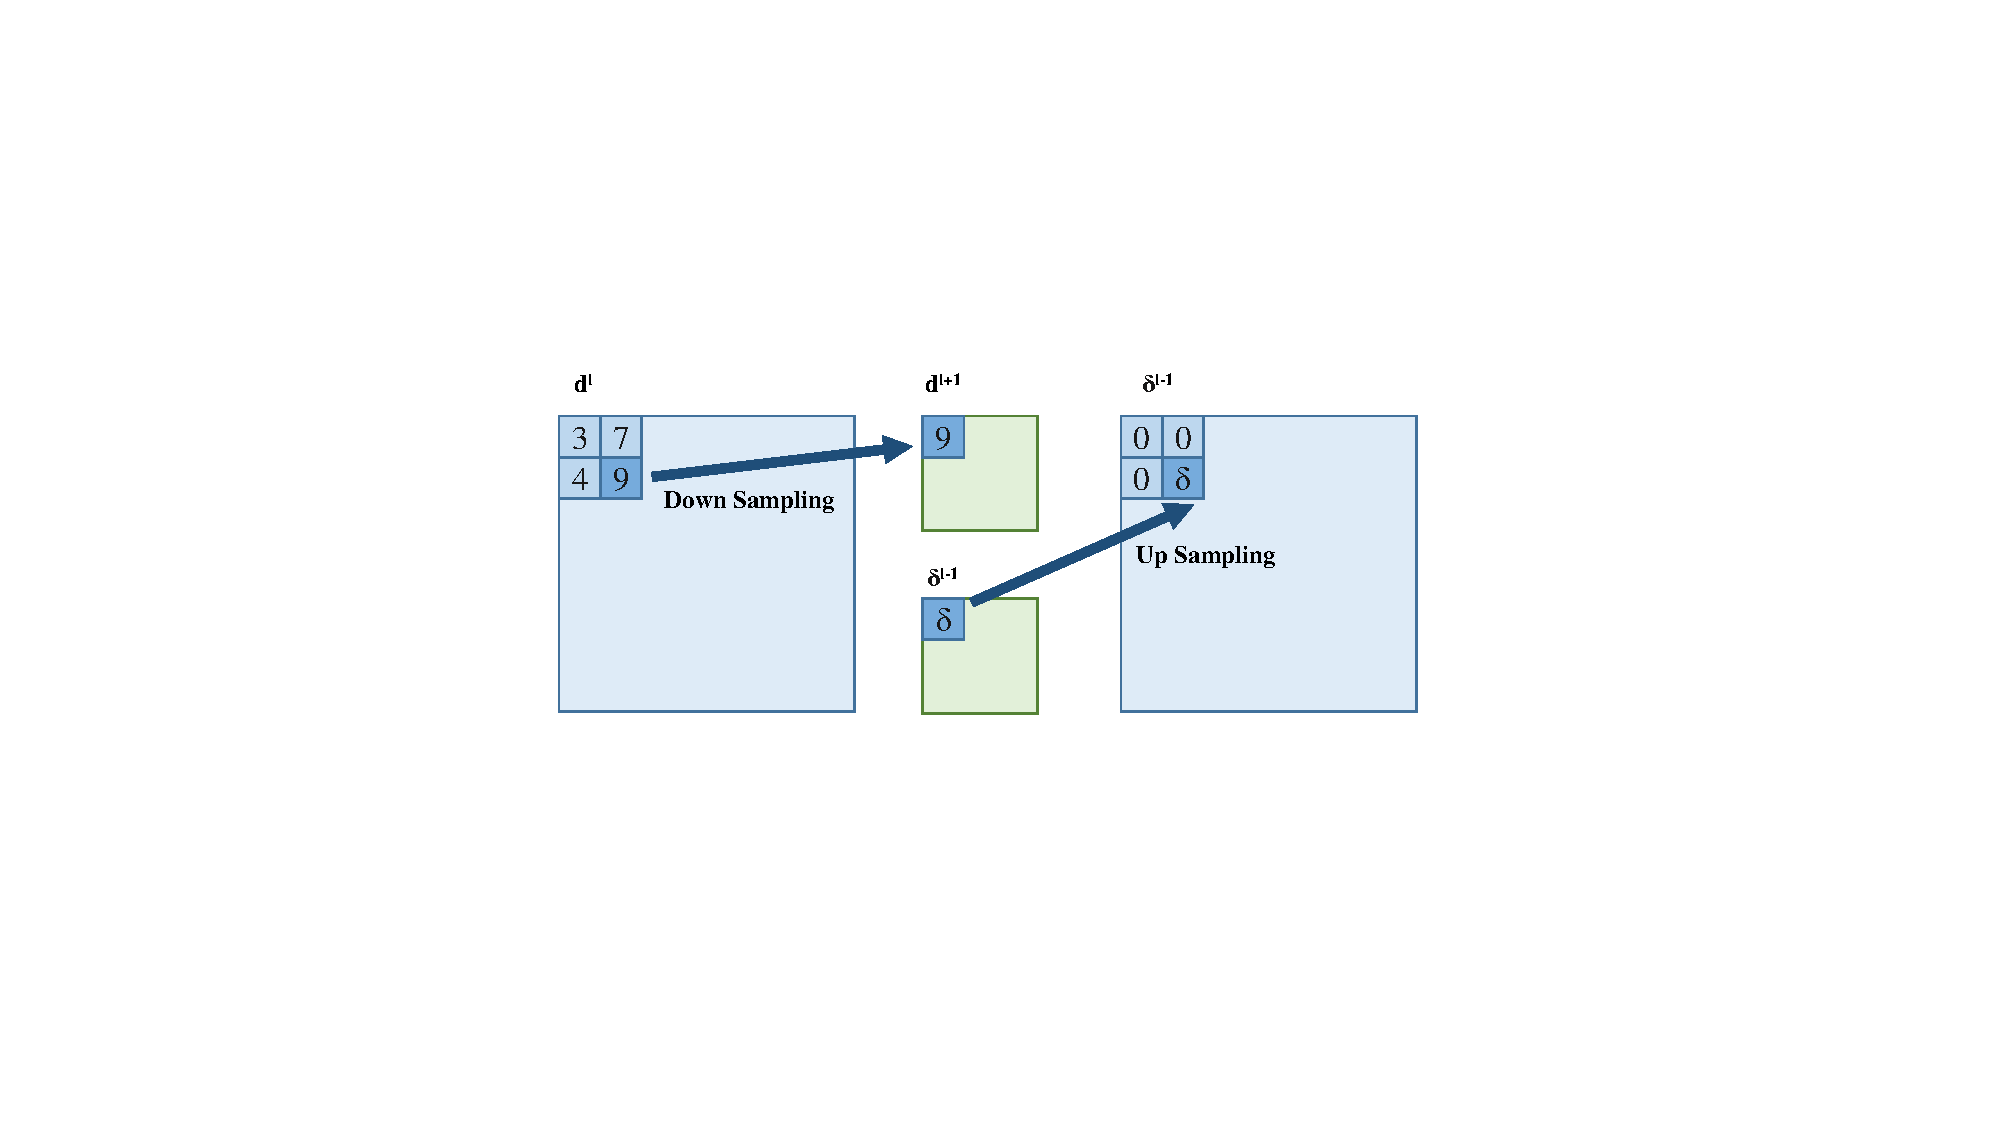
\includegraphics[width=3.2in]{figures/pool.pdf}
    \caption{Example of a $2\times 2$ max pooling layer}\label{fig:pool}
\end{figure}

\section{Hardware Friendly Training}\label{sec:training}

We first introduce two hardware-friendly training methods: fixed-point training and structured sparsity, followed by validating these methods on the real dataset.

\subsection{Fixed-point Data Based Training}
Traditional CNN training relies on full-precision data, i.e. 32-bit floating point data, to guarantee a good training accuracy. However, using fixed-point data in training process can help increase the energy efficiency of training. For CNN inference, varies accelerators have been proposed with fixed point operations to increase energy efficiency. For training, using fixed point data usually suffers great model accuracy loss. Recent work~\cite{zhou2016dorefa} use narrow bit-width only for data storage in training process but have to convert the data to floating point to process addition and multiplication. In this paper, we propose a training process using both fixed point format for data storage and computation. 

In the proposed training process, every fixed-point number is represented with low bit-width (e.g. 8 bit in our implementation) together with a scaling factor. We keep a common scale for each fixed-point blob, where a blob can be the activation of a layer, the weights of a layer, or the gradients of the weights/activations of a layer. Using this data format naively will induce two problems.

The first problem is how to convert the original floating point data to the fixed point version. This means to decide the scaling factor for each data blob. One choice is to use the dynamic range of each blob as the scaling factor can keep the data precision to the best degree, but this brings extra statistic and normalization operations for each data blob in each iteration. In this work, we focus on fine-tuning a pruned network. 
% \SH{don't let reviewers have the impression that you're bypassing the hardcore problem by fine-tuning.}
So we execute floating-point training iterations to analyze the dynamic scale of each blob and keep the scale through the rest of training process. Furthermore, we choose the nearest $2^n$ as the scaling factor which means data normalization can be implemented with shift operations on fixed-point data.

The second problem is the trade-off between bit-width and training accuracy. Low bit-width simplifies operations and reduce the storage consumption, but also reduce the model accuracy. For CNN training, the update step in each iteration is usually small because of small learning rate and gradient vanishing. Thus the update step is easy to underflow if using fixed point data with narrow bit-width.  In this work, we use narrow bit-width for activations and gradients. Because the scaling factor of gradient blob can be much smaller than that of weights, we use a larger bit-width to avoid gradient underflow when the gradients and weights are to be aligned and added together. To reduce the hardware cost for each operation, we only use the MSBs of weights to execute feed forward and back propagation.

An example of the proposed fixed-point based training process is shown in Figure~\ref{fig:train_fixed}. The right part of the figure shows the feed forward phase of the network from top to bottom while the left part shows the back propagation phase from bottom to top. The learning rate is merged with the scaling factor and converted to shift operation before computing $\Delta W$ and $\Delta B$. Currently, weight decay and momentum are not supported in our hardware design. So we also omit these two functions in our software experiments. These two functions will not greatly affect hardware design and are to be supported in the future.

\begin{figure}[tb]
  \centering 
  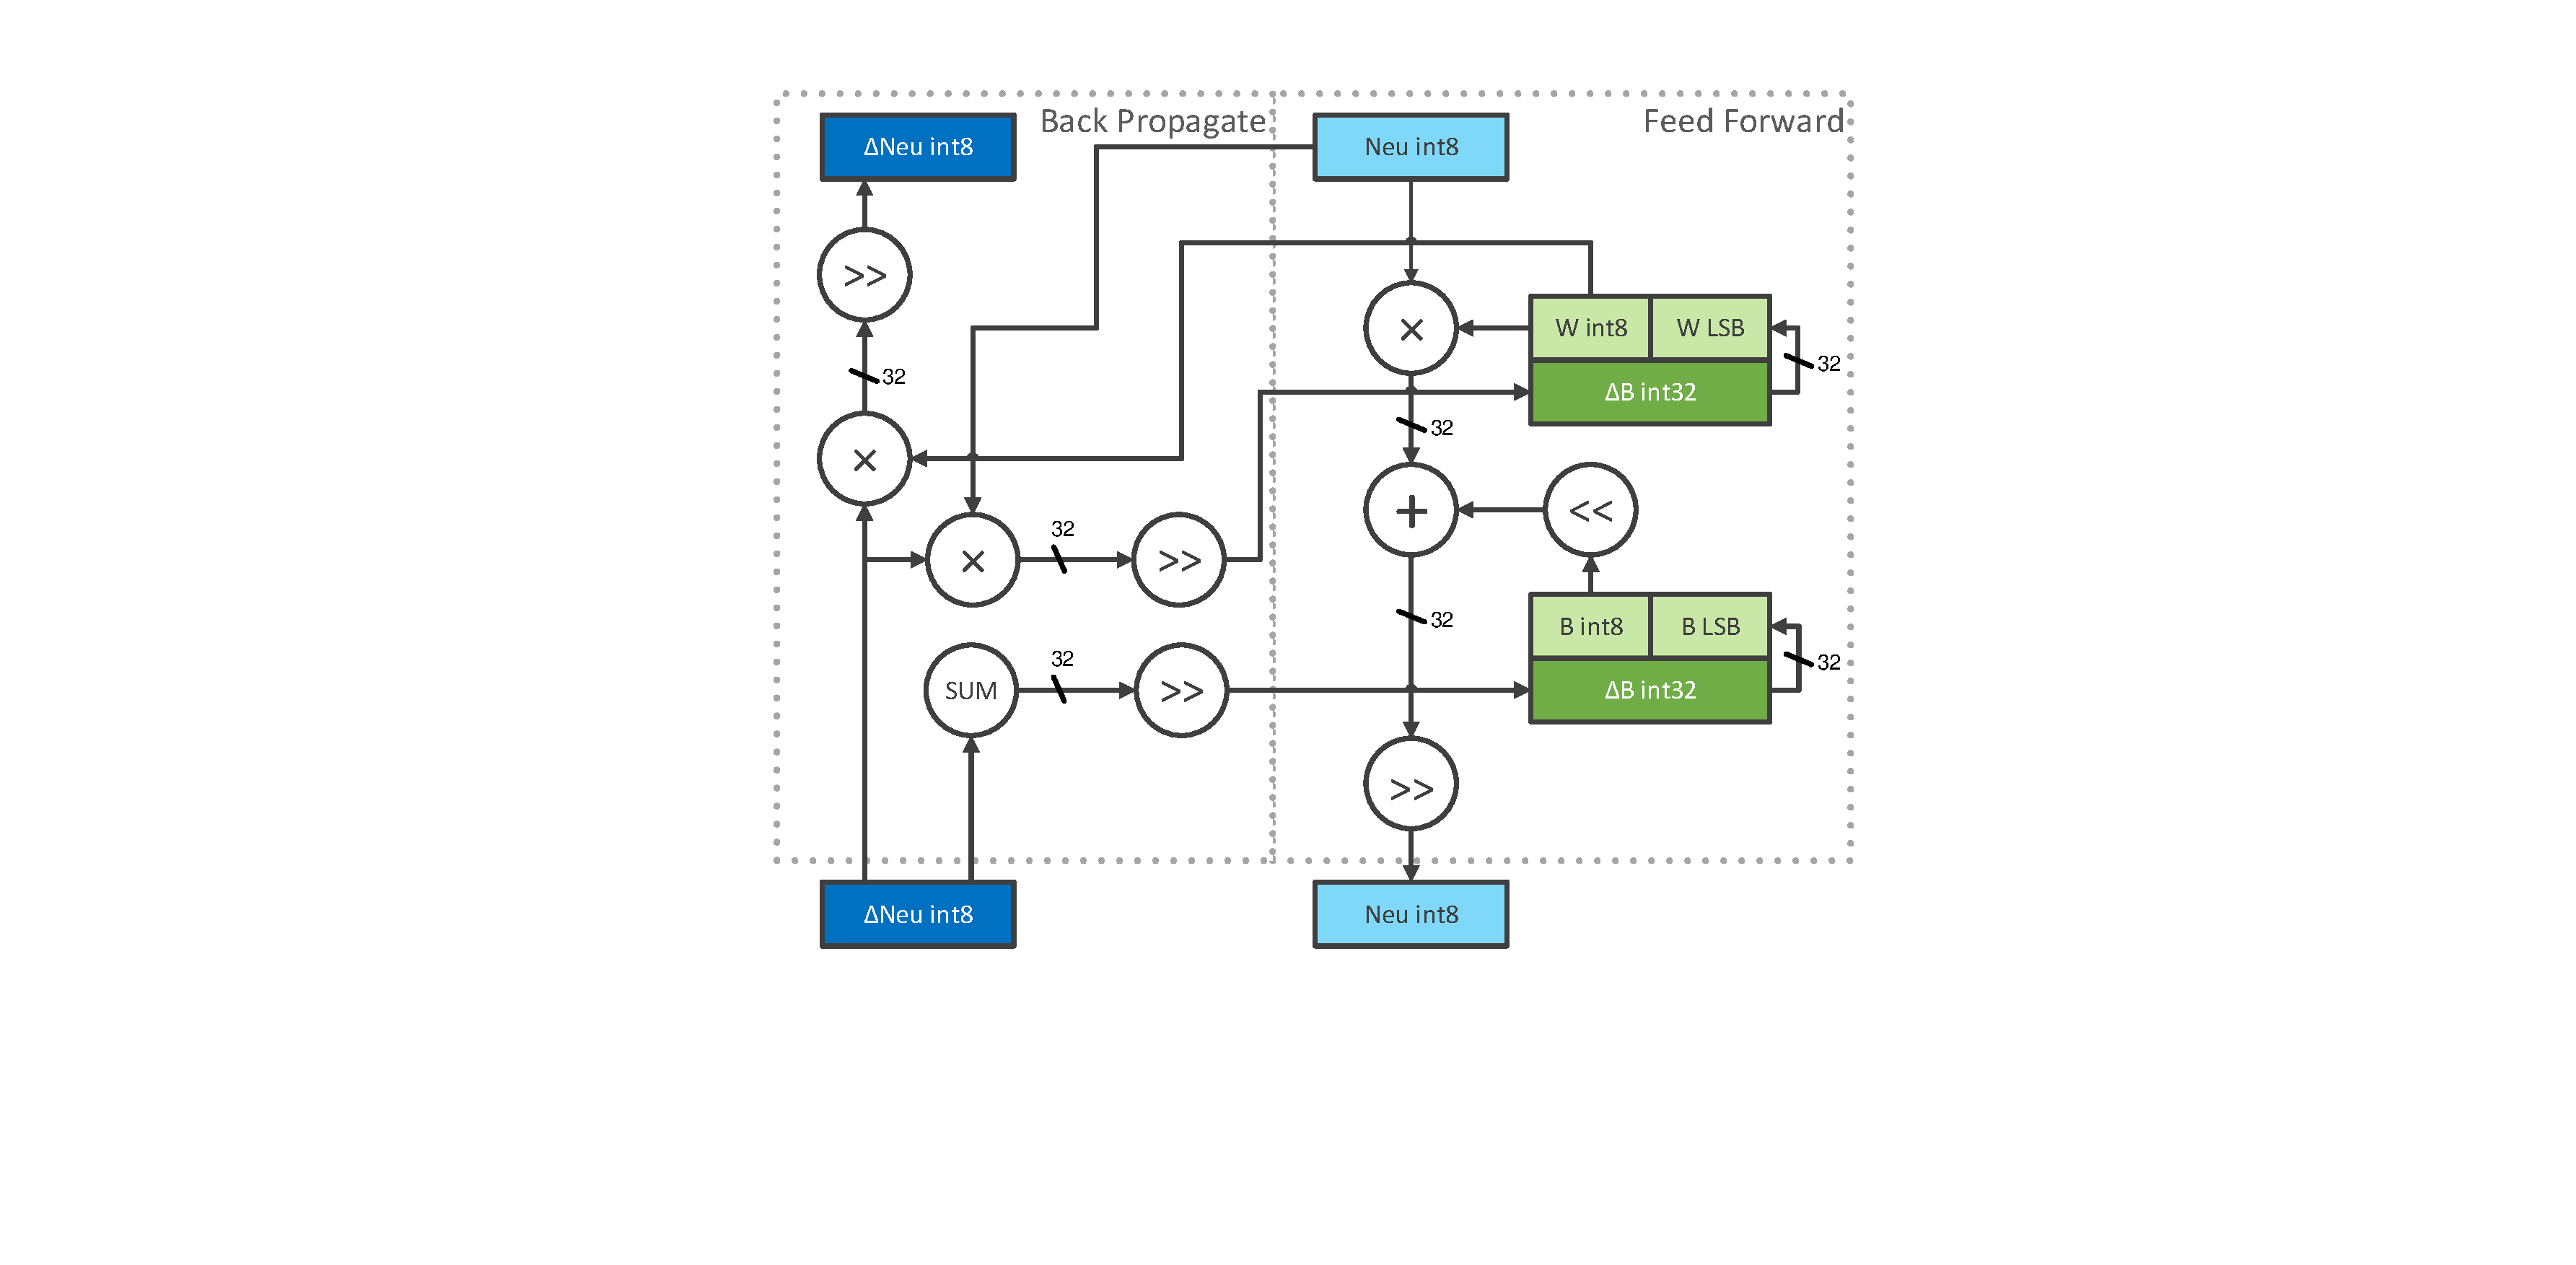
\includegraphics[width=1.0\columnwidth]{figures/train_fixed.pdf}
  \caption{An example of the proposed training process with 8-bit for neuron and weight MSB and 24bit for weight LSB buffer. }
  \label{fig:train_fixed}
\end{figure}

\subsection{Structured Pruning}

We denote shape of weights as $(N, C, H, W)$. $N$ represents output channel, $C$ represents input channel, $H$ represents height, and $W$ represents weight. Compared to element-wise pruning, group-wise pruning is more efficient for hardware to realize. We choose kernel-dim pruning, which means the atomic elements during pruning is $H \times W$. L2-norm of the atomic elements is calculated, and atomic elements with small l2-norm are pruned. Mask matrix is used to label where is pruned and has the same shape as weights. If the weight is pruned, its mask becomes 0. Then we get sparse weights and mask matrix. 

\begin{figure}[tb]
    \centering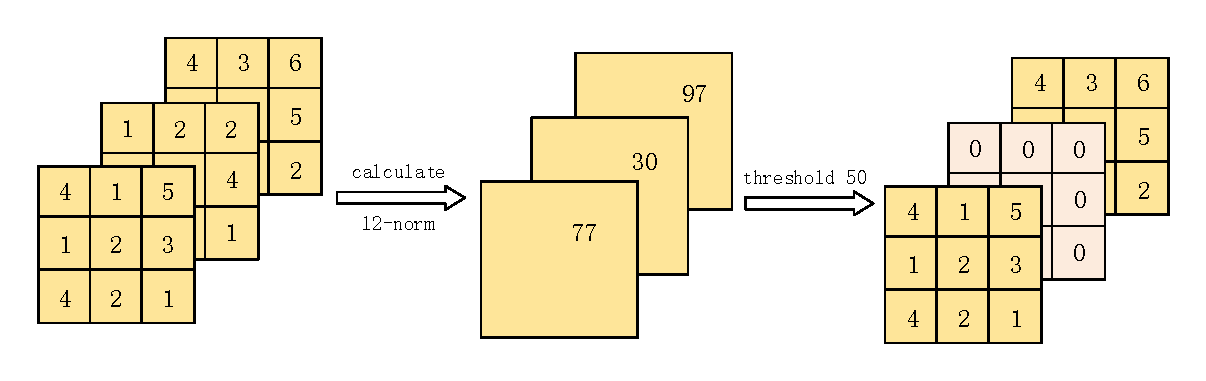
\includegraphics[width=3.5in]{figures/prune-light.pdf}
    \caption{Illustration of the group-wise pruning}\label{fig:prune}
\end{figure}

\begin{table}[tb]
\centering
\caption{Structure of the neural network for the experiment. Sparsity denotes the ration of zeros element or convolution kernel in a layer.}
\label{table:sparsity}
\begin{tabular}{|c|c|c|c|}
\hline
Layer    & Type                                                  & \begin{tabular}[c]{@{}c@{}}Dimenson\\ (NxCxHxW)\end{tabular} & Sparsity \\ \hline
conv1    & conv                                                  & 64x3x3x3                                                   & 0.1      \\ \hline
pool1    & \begin{tabular}[c]{@{}c@{}}max\\ pooling\end{tabular} & -                                                            & -        \\ \hline
conv2    & conv                                                  & 128x64x3x3                                                   & 0.4      \\ \hline
pool2    & \begin{tabular}[c]{@{}c@{}}max\\ pooling\end{tabular} & -                                                            & -        \\ \hline
conv3\_1 & conv                                                  & 256x128x3x3                                                  & 0.3      \\ \hline
conv3\_2 & conv                                                  & 256x256x3x3                                                  & 0.4      \\ \hline
pool3    & \begin{tabular}[c]{@{}c@{}}max\\ pooling\end{tabular} & -                                                            & -        \\ \hline
conv4\_1 & conv                                                  & 512x256x3x3                                                  & 0.5      \\ \hline
conv4\_2 & conv                                                  & 512x512x3x3                                                  & 0.7      \\ \hline
pool4    & \begin{tabular}[c]{@{}c@{}}max\\ pooling\end{tabular} & -                                                            & -        \\ \hline
conv5\_1 & conv                                                  & 512x512x3x3                                                  & 0.9      \\ \hline
conv5\_2 & conv                                                  & 512x512x3x3                                                  & 0.9      \\ \hline
pool5    & \begin{tabular}[c]{@{}c@{}}max\\ pooling\end{tabular} & -                                                            & -        \\ \hline
dense6   & fc                                                    & 512x512                                                      & 0.9      \\ \hline
dense7   & fc                                                    & 512x512                                                      & 0.9      \\ \hline
dense8   & fc                                                    & 512x10                                                   & 0.9          \\ \hline 
\end{tabular}
\end{table}


\subsection{Software Validation}

The whole training process used in this work is as follows:
\begin{itemize}
\item Training a fixed-point model with fixed-point weights and activations using full-precision gradients on software.
\item Pruning weights and getting the mask matrix.
\item Training a fixed-point model on hardware using fixed-point gradients while keeping pruned weights zero.
\end{itemize}

The first two steps are implemented with software which use CPU and GPU as the computation platform. The third step can be executed with the proposed hardware architecture. To test the performance of the fixed-point based training method, we implemented a software version of the fixed-point data based CONV, ReLU, and pooling layers on TensorFlow.

In our implementation, the bit width of the weight buffer is set to be 24bit. The fixed scale of every gradient accumulation buffer is decided using the weight scale, the gradient scale and the learning rate after the first step. In this fine-tune stage, the fixed scales for every weight/activation/gradient blobs are fixed, and no momentum or weight decay is used. This ensures that every detail will be the same as the hardware implementation.

We perform the experiment using VGG-11\cite{Simonyan2014Very} on CIFAR-10\cite{krizhevsky2009learning} dataset. While training in the first step, the learning rate is set to 0.05 and decayed by 0.5 every 30 epochs; weight decay is set to $5 \times 10^{-4}$ and momentum is set to 0.9. We pruned model to the same sparsity in the whole experiments shown in Table~\ref{table:sparsity}. In the third training step with fixed point data, we compare the result of training with and without momentum. The accuracy is nearly the same(90.54 vs. 90.53). 

Furthermore, we also evaluate where is a good point to stop floating point training and starts fixed point training with pruned weights. Usually, we prune model when it is perfectly trained and achieves the best accuracy. But if we want to save the training time, we do not need to prune model until it perfectly trained. Table~\ref{table:prune} shows experimental results for pruning at different training stages. 

\begin{table}[tb]
\centering
\caption{Comparison of training result with different number of initial epochs before training}
\label{table:prune}
\begin{tabular}{ccccc}
\hline
\begin{tabular}[c]{@{}c@{}}Initial\\ accuracy\end{tabular} & \begin{tabular}[c]{@{}c@{}}Initial\\ epochs\end{tabular} & \begin{tabular}[c]{@{}c@{}}Fine-tune\\ Accuracy\end{tabular} & \begin{tabular}[c]{@{}c@{}}Fine-tune\\ epoches\end{tabular} & \begin{tabular}[c]{@{}c@{}}Total\\ epoches\end{tabular} \\ \hline
90.98                                                      & 220                                                       & 90.81                                                        & 100                                                         & 320                                                     \\
90.05                                                      & 130                                                       & 91.11                                                        & 200                                                          & 330                                                     \\
89.58                                                      & 100                                                        & 91.01                                                        & 195                                                         & 295                                                     \\
88.06                                                      & 65                                                        & 90.54                                                        & 130                                                         & 195                                                     \\
85.50                                                      & 45                                                        & 90.05                                                        & 115                                                         & 160                                                     \\\hline
\end{tabular}
\end{table}

The result in Table~\ref{table:prune} shows that, if we start pruning at half of training, it may cost less epochs without harming accuracy, even with small accuracy improvement. The best accuracy occurred having 130 epochs of dense training and 200 epochs of sparse training. The stopping criteria is when the learning curve starts to flatten. In this training task, 200 out of 330 epochs can be accelerated with hardware.


\section{Hardware Design}\label{sec:hw}

\begin{figure*}[t]
  \centering
  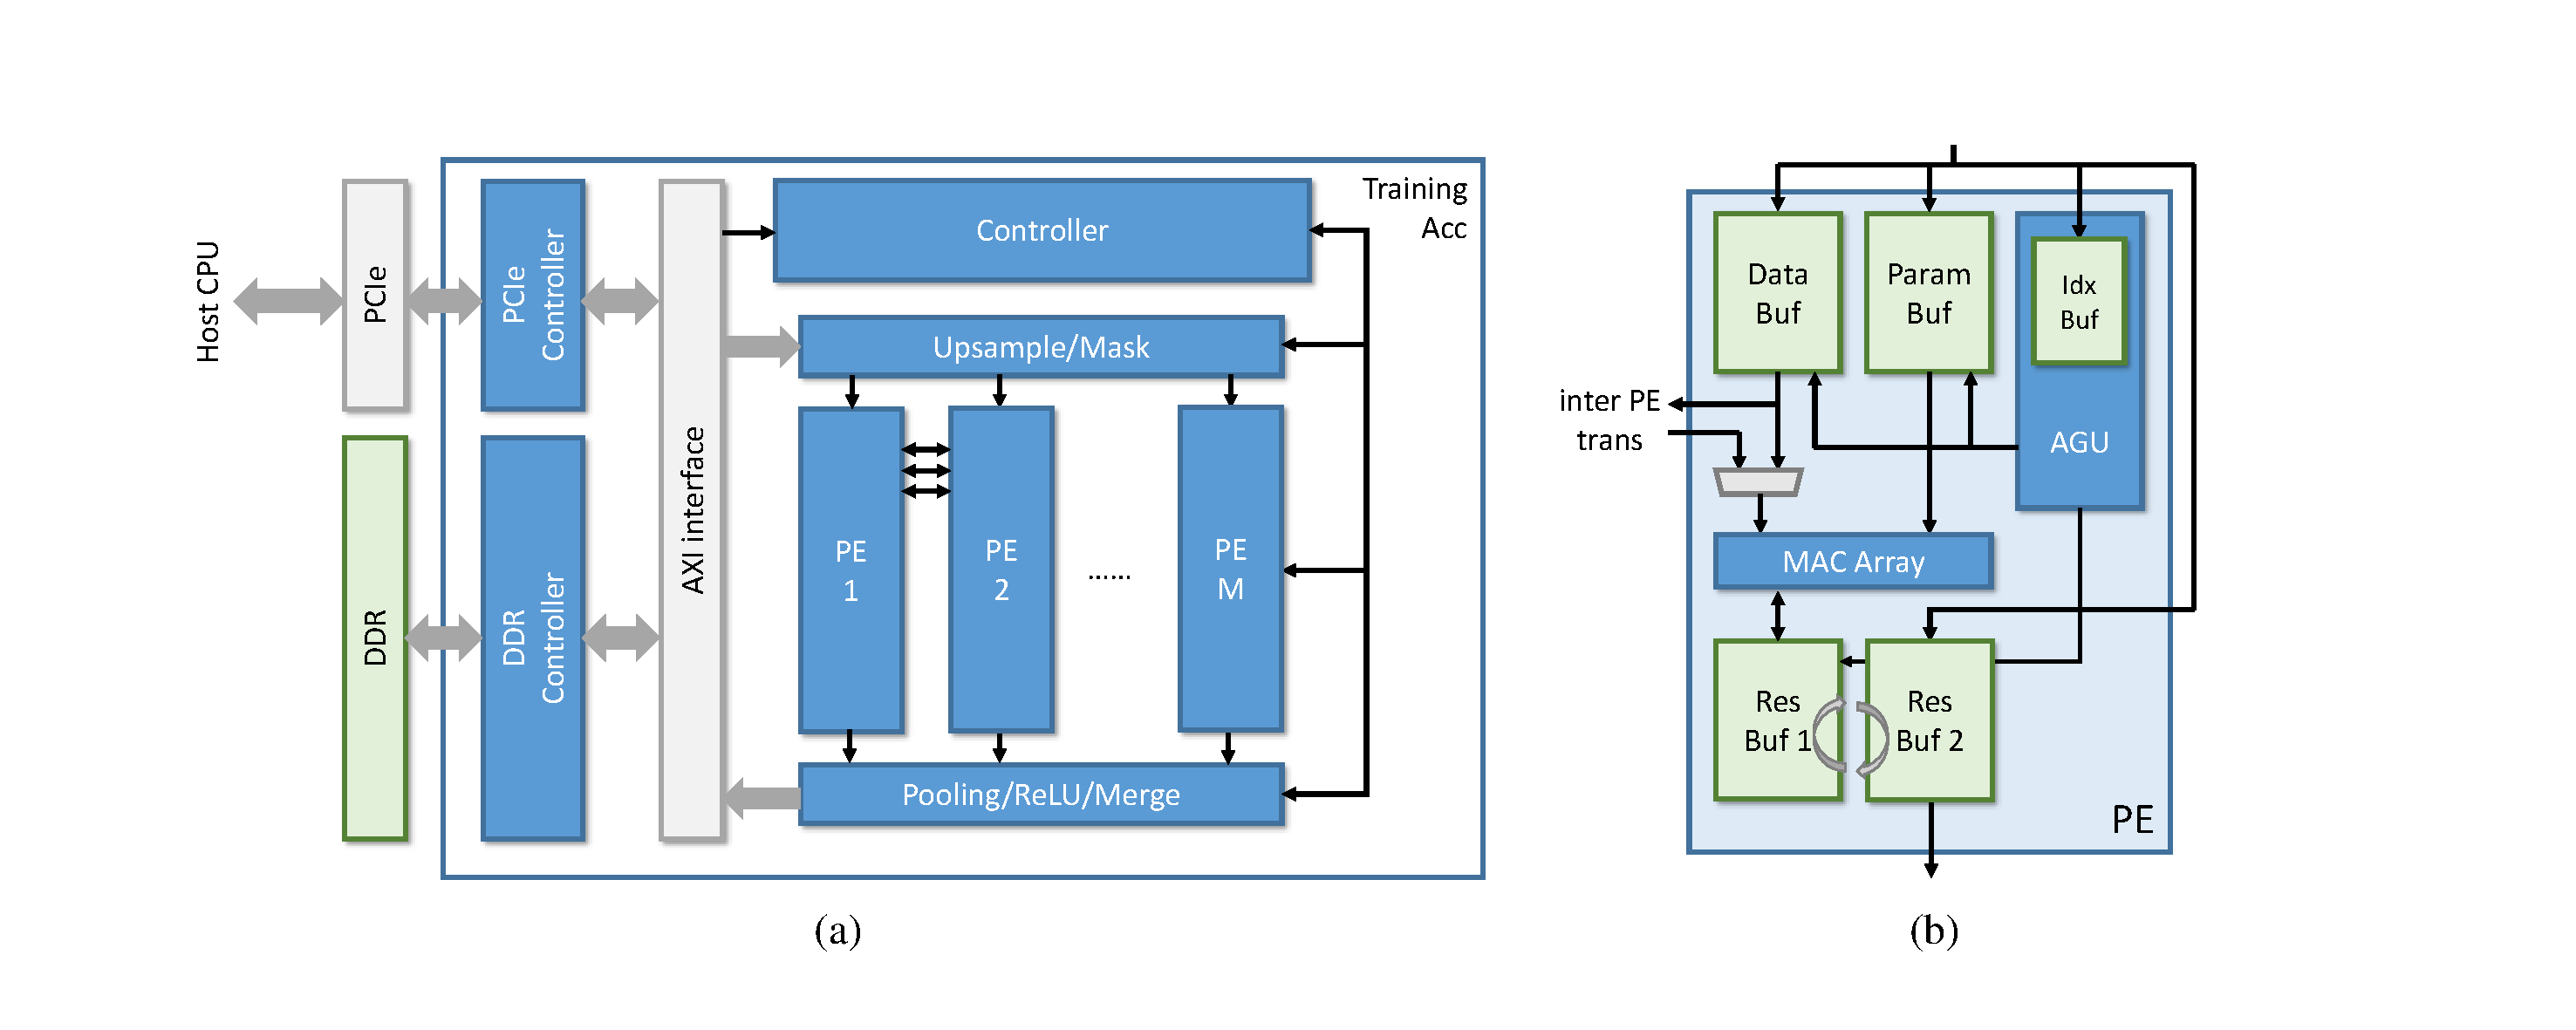
\includegraphics[width=2\columnwidth]{figures/architecture.pdf}
  \caption{The CNN training accelerator architecture. (a) The overall system architecture. (b) The structure of a single PE. }
  \label{fig:arch}
\end{figure*}

In this section, we introduce the hardware design for training CNN with sparse parameters. Especially, we will show architecture support for sparse operations and how this design differ from inference accelerators.

\subsection{Overall Architecture}
Figure~\ref{fig:arch}(a) shows the overall architecture of the hardware design. 
% \SH{seems to be the same as the FPGA'16 figure; there's not much information in this figure.}
% below are redundant for ISCA:
% The proposed architecture serves as an accelerator for a CPU host system.
% The accelerator is connected with the host CPU through the PCIe interface. 
When the accelerator works, the host CPU sends a mini-batch of training data to the accelerator to process an iteration of training. The accelerator first processes inference on the mini-batch and sends back the result vector to CPU to calculate the loss. After that, the gradient vector of the last layer is given back to the accelerator to do back propagation. This process
 is iteratively executed until training converges.

External memory are implemented to meet the large storage requirement of training. Compared with inference, the feed-forward results of each layer of the mini-batch should be kept until back propagation is done. Though we use fixed-point data for training, the training on a mini-batch still requires GB level of memory, which is impractical to be stored on-chip. A set of on-chip buffers are implemented to explore the spatial locality of convolution operation and allows fast irregular data access for sparse operations. Details of each PE will be introduced in section~\ref{sec:hw_pe}.

The CNN layers are executed on the hardware layer by layer. For pooling and ReLU layers, the FF, NG and WG stages are all implemented as a pipeline stage after or before PE. Because pooling and ReLU layers has little workload, the functions are implemented as common modules for all the PEs and can be bypassed if necessary. For each layer, the data is first loaded from DDR and is sent to the Upsample/Mask unit. In inference phase, the data is directly issued to corresponding PEs. In back propagation phase, upsampling and mask function is applied on the activation data. Then in each PE, the calculation of the nested loops are processed. Then the results are sent to Pooling/ReLU/Merge unit where the pooling and ReLU function is applied as traditional CNN inference accelerator design. The merge function adds gradient result from different PEs during back propagation phase.

\subsection{PE for Sparse Computation}\label{sec:hw_pe}

\begin{figure}[htb]
  \centering
  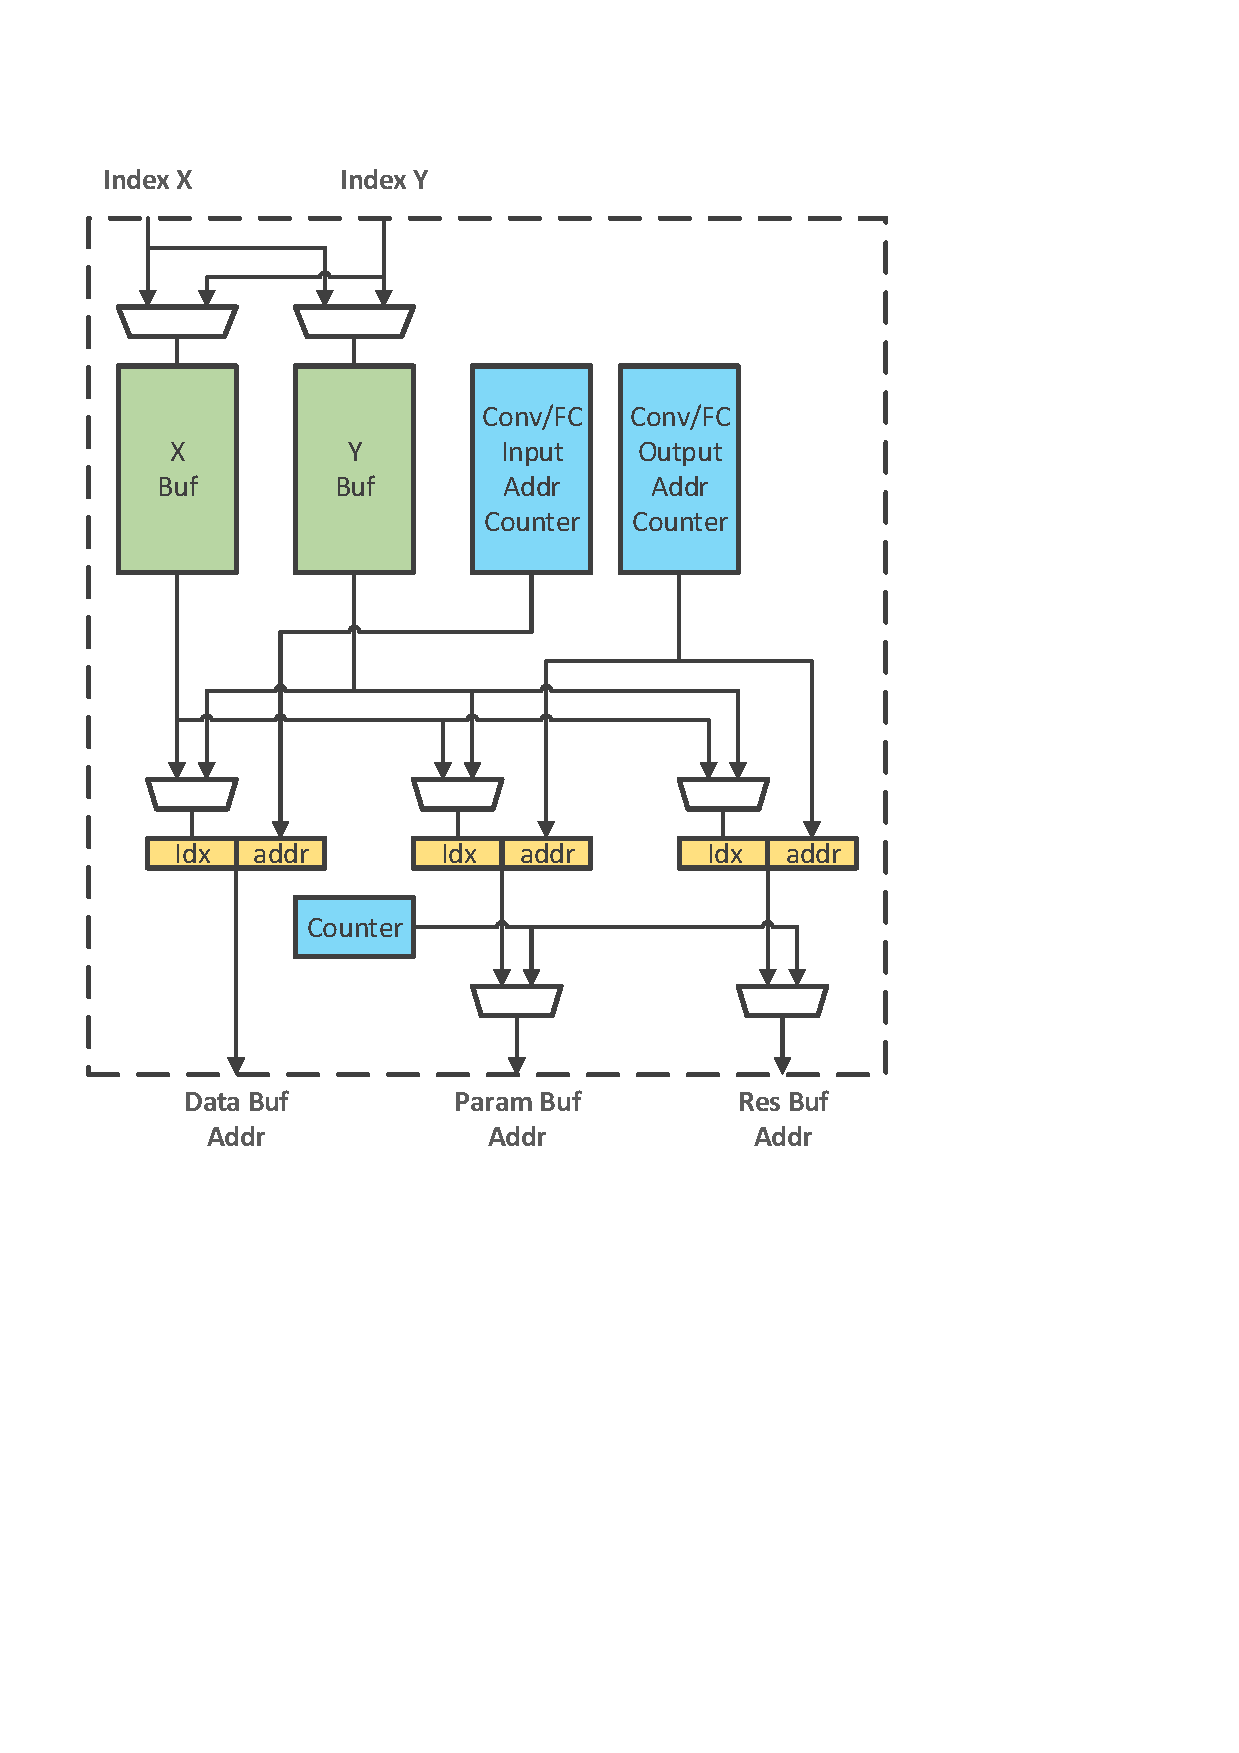
\includegraphics[width=1.0\columnwidth]{figures/agu.pdf}
  \caption{AGU architecture.}
  \label{fig:agu}
\end{figure}

To fully take advantage of the sparse weights in training, the hardware should support the following two types of sparse operations:
\begin{itemize}
\item $D\times S=D$: For FF and NG steps, the neurons or neuron gradients are multiplied with the sparse weights to get the neuron of next layer or the gradient of the previous layer. So one of the two operators for multiplication is sparse.
\item $D\times D=S$: For wG steps, the neurons are multiplied with the back propagated neuron gradients to get the weight gradients. Both the operators of multiplication are dense but the result is sparse.
\end{itemize}

\begin{figure*}[t] 
  \centering
  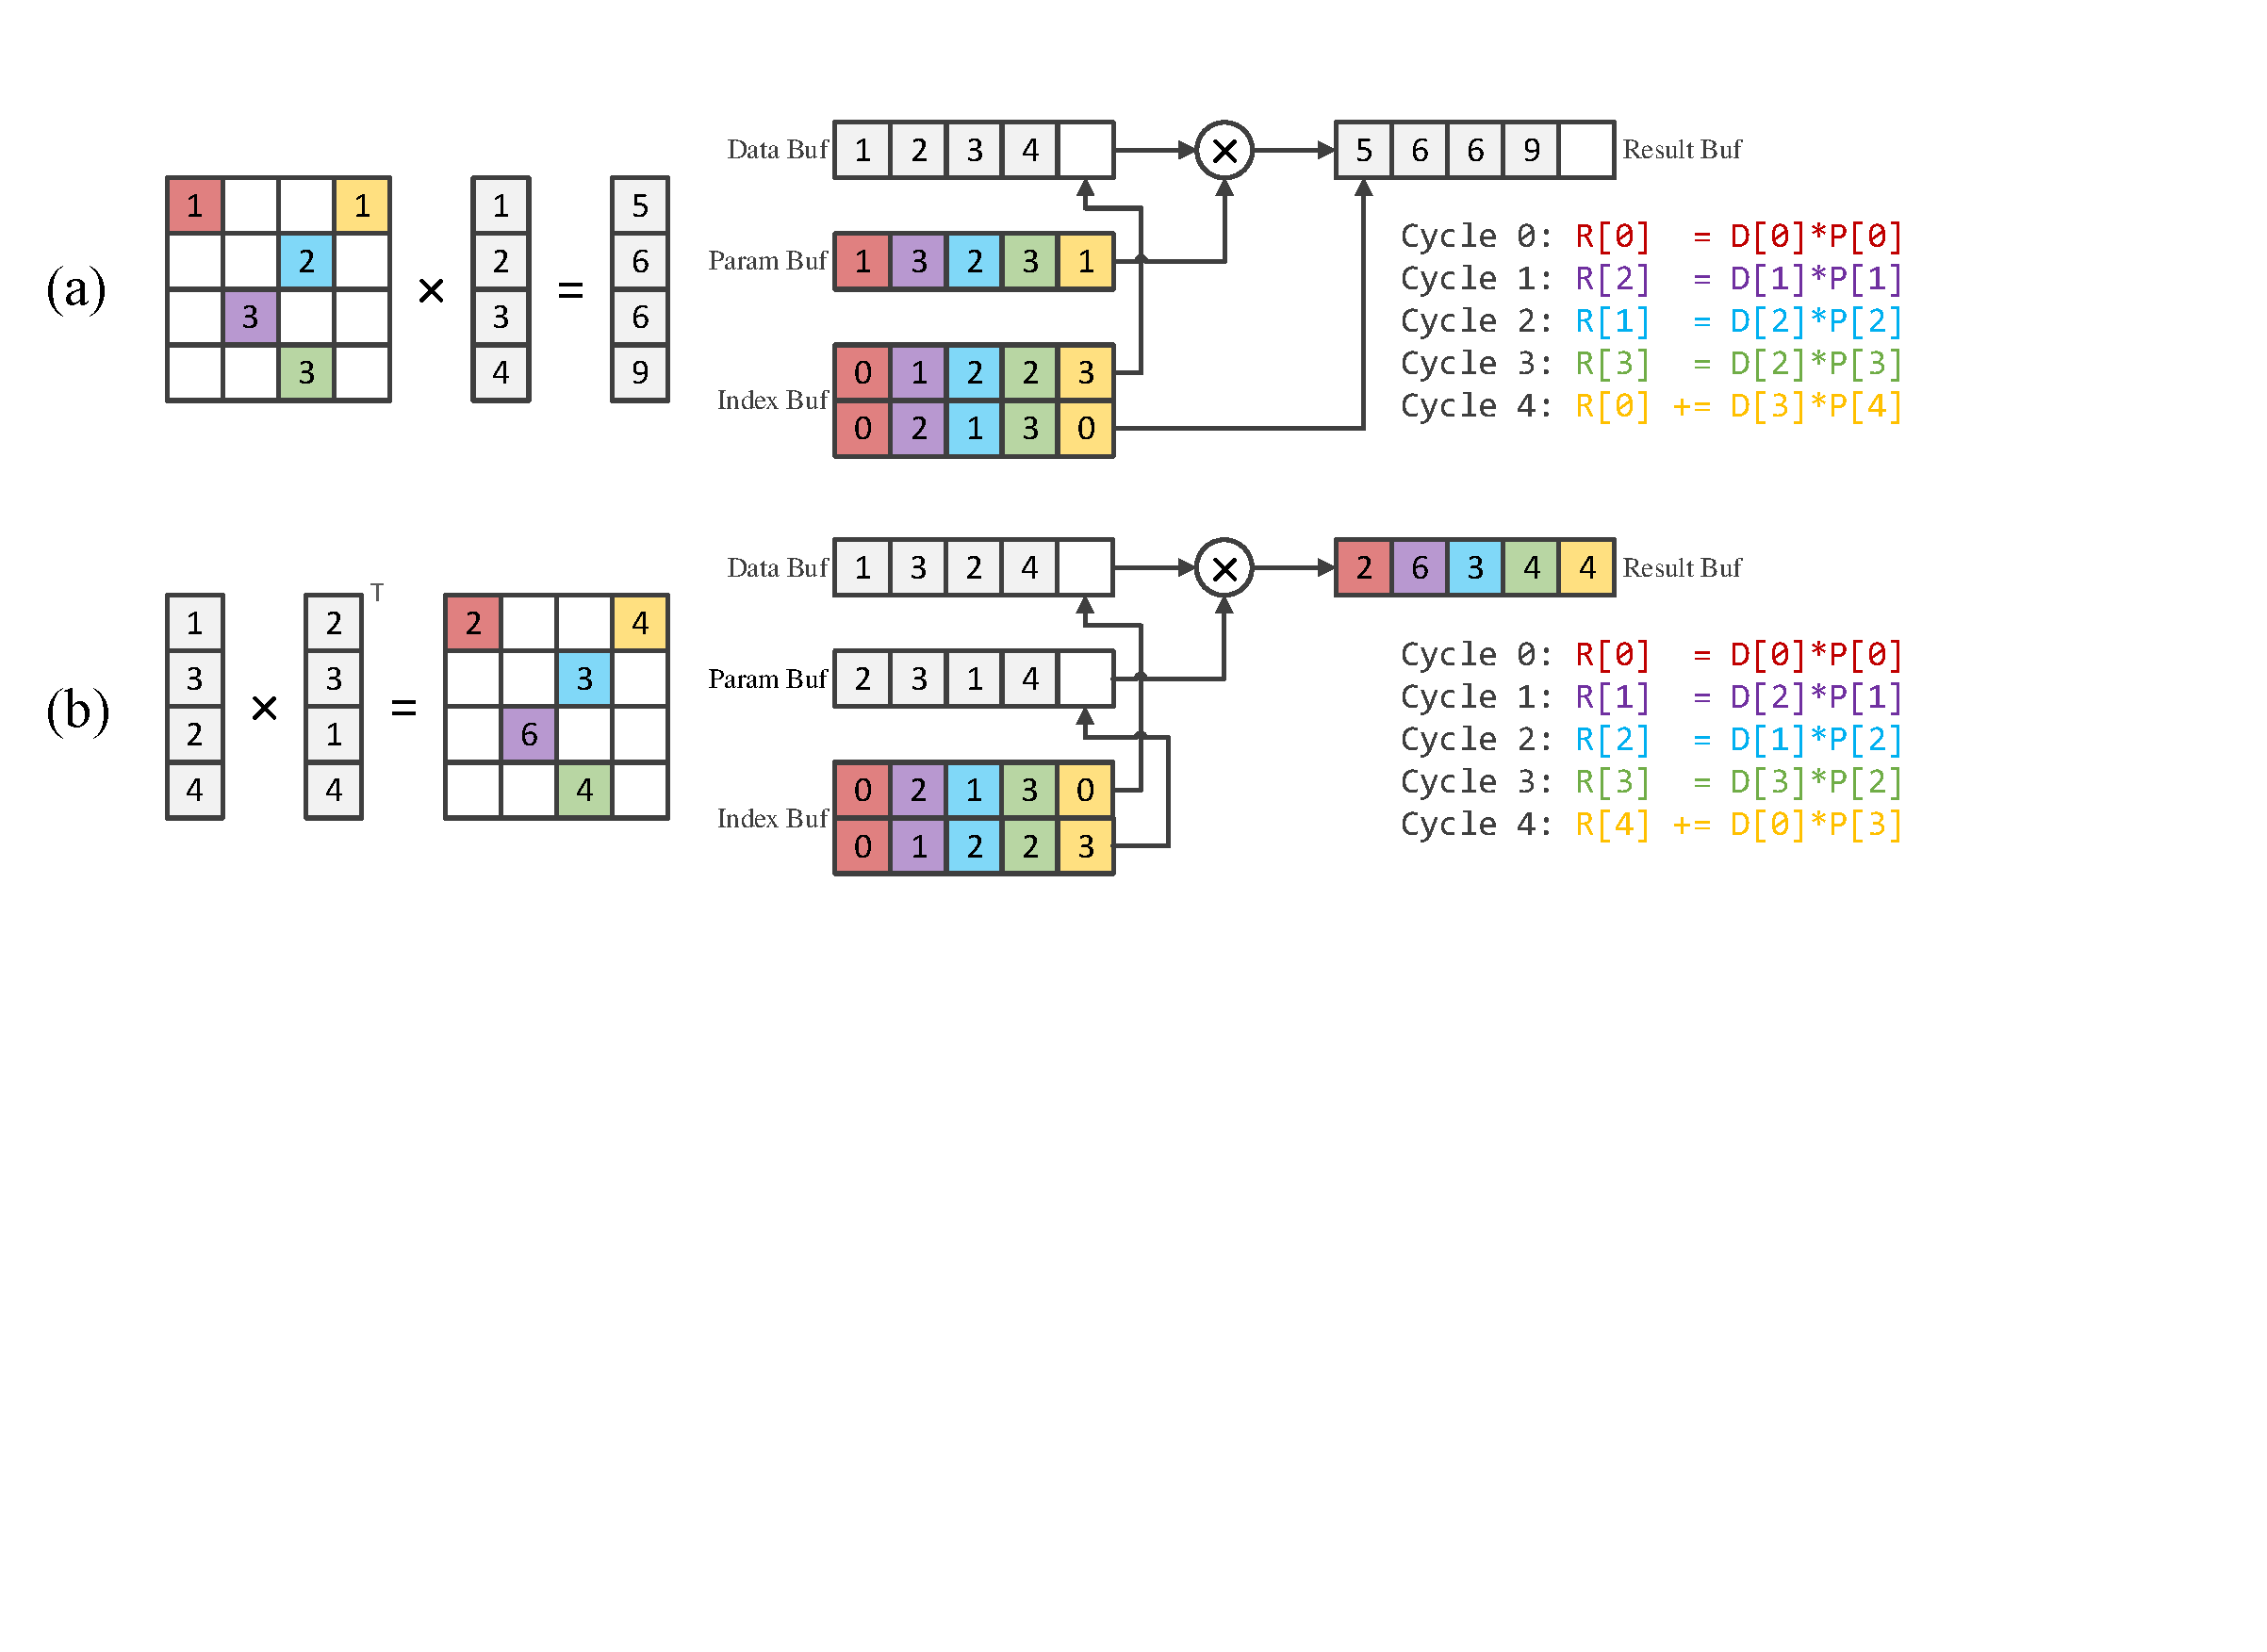
\includegraphics[width=1.8\columnwidth]{figures/sparse_mv.pdf}
  \caption{The hardware behavior for sparse network process. (a) Sparse matrix vector multiplication for inference and calculation of gradient of activations. (b) Vector vector multiplication to calculate the gradient of sparse parameters. }
  \label{fig:spmv}
\end{figure*}


We choose to process the sparse computation in a block manner. In this manner, the hardware can support both of the sparse operation types efficiently. An example of a $4\times 4$ block of fully connected layer executed in a PE is shown in Figure~\ref{fig:spmv}. Each weight matrix element is stored with its relative 2-D position in the block. Each time a pair of index $(x, y)$ is fetched from the index buffer. For inference, as shown in Figure~\ref{fig:spmv}(a), $x$ is used to access the activations in data buffer and $y$ is used to access the result. To calculate the gradient of the sparse parameters, data buffer and parameter buffer store the activation of two adjacent layers. $x$ and $y$ are used to access the buffers respectively. Different PEs work independently on different blocks for higher parallelism.

Note that for the case in Figure~\ref{fig:spmv}(a), changing the order of indexes in index buffer will not change the result, as long as the order of indexes corresponds to that of the parameters. This property is also true for Figure~\ref{fig:spmv}(b). So in NG step, when we need to use a transpose format of the weight matrix, we only need to exchange $x$ and $y$ with a hardware multiplexer and do not need to change the data format in external memory as suggested in Section~\ref{sec:prelim:fc}. 

For CONV layers, as the sparsity is 2-d kernel level structured, the same sparsity is also supplied. If we replace the entries in the matrix with 2-d convolution kernels, each element in vector as a feature map, and scalar multiplication with 2-d convolution, the above example becomes a CONV layer example.

The structure of each PE is shown in Figure~\ref{fig:arch}(b). Similar to the example in Figure~\ref{fig:spmv}, we implement {\bf{DataBuf}} for neuron(feature map), {\bf{ParamBuf}} for weights(convolution kernels) and {\bf{ResBuf}} for neuron(feature map) with on-chip RAM. {\bf{DataBuf}} and {\bf{ParamBuf}} are in simple dual port mode and works in a ping-pong manner by spliting the address space. {\bf{ResBuf}} is implemented with two simple dual port RAMs because accumulation function requires extra RD/WR port.

The detail of the address generation unit(AGU) is shown in Figure~\ref{fig:agu}. AGU implements {\bf{XBuf}} and {\bf{YBuf}} to store the relative index of each weights or convolution kernel within a processing block. We use a multiplexer on the write port of the buffer to support transpose function. For the buffers to be randomly accessed, the X and Y index read from index buffer directly serve as the high bits of RAM addresses, which help to select the channel or neuron to use. An index independent counter helps generate the address sequence to carry out 2-d convolution for CONV layer or scaler multiplication for FC layer. For the buffer to be sequentially accessed, another counter is used generate address sequence.

\subsection{Loop Unrolling Strategy}\label{sec:hw_unroll}
\begin{figure*}[t]
  \centering
  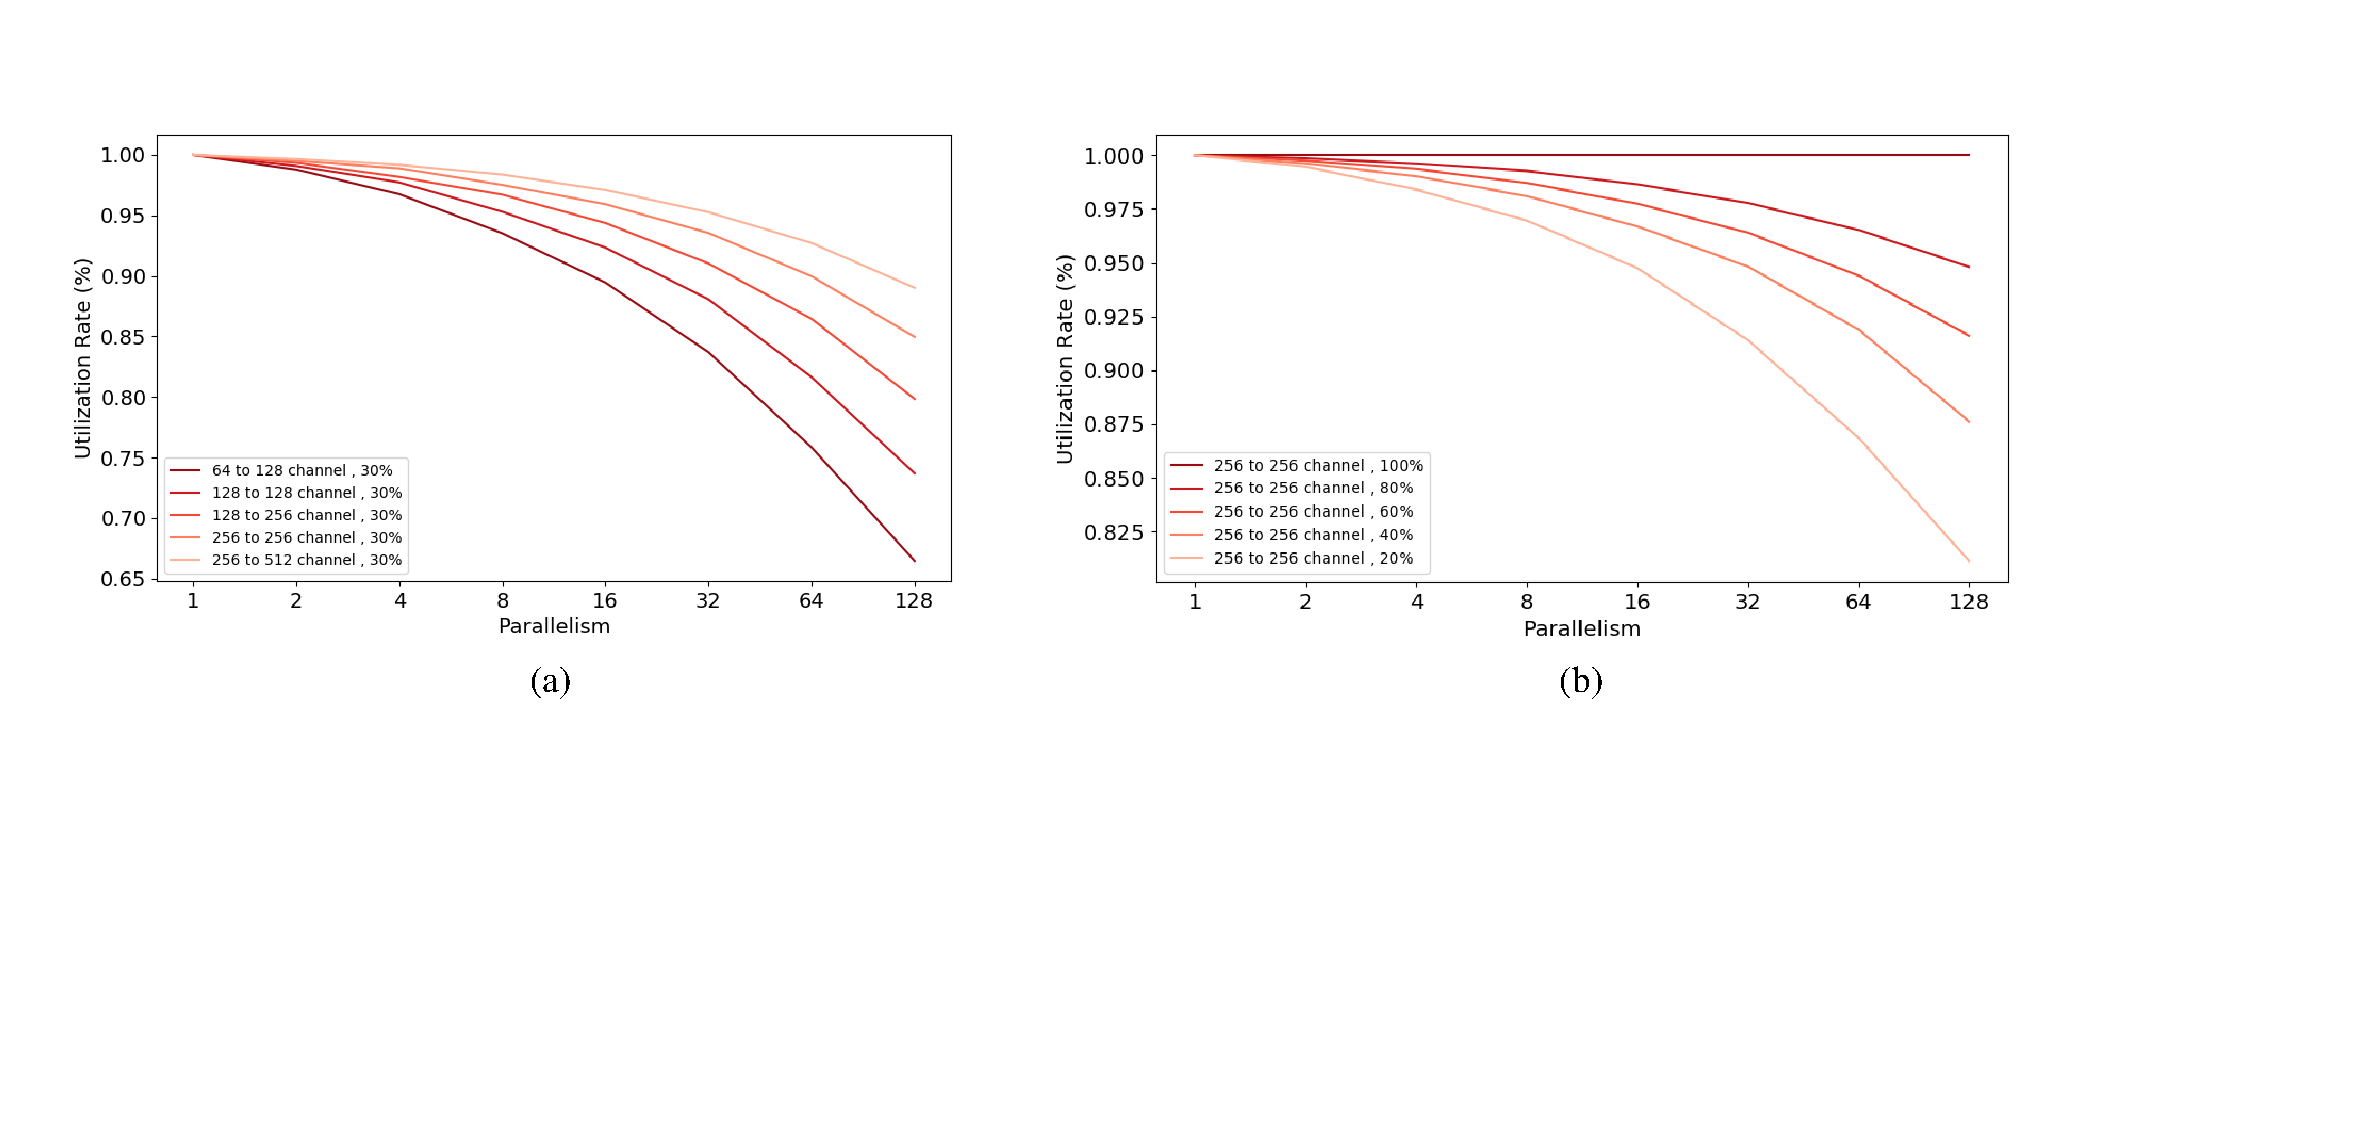
\includegraphics[width=2.0\columnwidth]{figures/util_sim.pdf}
  \caption{Hardware utilization ratio under different sizes of sparse parameters and sparsity. (a) Estimation with a fixed sparsity and different parameter scales. (b) Estimation with a fixed parameter size and different sparsities.}
  \label{fig:util_sim}
\end{figure*}

There is already enough discussions on how to unroll the loops on hardware for CNN inference with dense models~\cite{zhang2015optimizing,mao2017exploring}. But for back propagation and sparse model, the strategy should be different. Here, we analyze different unroll dimensions one by one.

{\bf{Batch}}. Parallelism in batch dimension will not affect hardware design compared with inference accelerator. For training, usually a mini-batch is used in each iteration. So parallelism in batch is always preferred.

{\bf{Layer}}. Parallelize the process of different layers means pipeline different layers. For CNN training, the result of processing one mini-batch is necessary for the next one. So implementing a long pipeline will cause large overhead between the process of adjacent mini-batches. This dimension is not preferred.

{\bf{Input/output channel}}. The unroll parameter in these two dimensions are limited by network sparsity. This is caused by workload imbalance. For example, for a CONV layer, unroll the output channel with M means splitting the workload to M different hardware unit to process in parallel. Because the network is structured sparse, the number of 2-d convolution kernels for each hardware unit to process may different. Some experiments are carried out to show the parallelism affects the hardware utilization ratio as shown in Figure~\ref{fig:util_sim}. In Figure~\ref{fig:util_sim} (a), we suggest that the parameters are uniformly distributed with the density of $30\%$ and varies the size of parameter. It is clear to see that to keep the utilization ratio, we should choose smaller parallelism for a smaller parameter size. In Figure~\ref{fig:util_sim} (b), we keep the parameter size and changes the sparsity. For parameters with less non-zero values, we need to use a smaller parallelism to get the same hardware utilization ratio.

{\bf{Feature map}}. Unrolling in feature map means computing multiple output feature map pixels in parallel. If the output of 2-d convolution is comparable or even smaller than the unroll factor, there will be hardware overhead. For training of CONV layers, the WG steps can be expressed as the 2-d convolution of the input feature map with the gradient of the output feature map. The convolution output size is the same as the convolution kernel, which is usually as small as $3\times 3$. So the unroll factor should be carefully chosen.

{\bf{Convolution kernel}}. Unrolling convolution kernel dimension is faced with the same problem as that of unrolling feature map, not in WG steps, but in FF and NG steps. So the unroll factor should be carefully chosen.

\begin{figure*}[t]
  \centering
  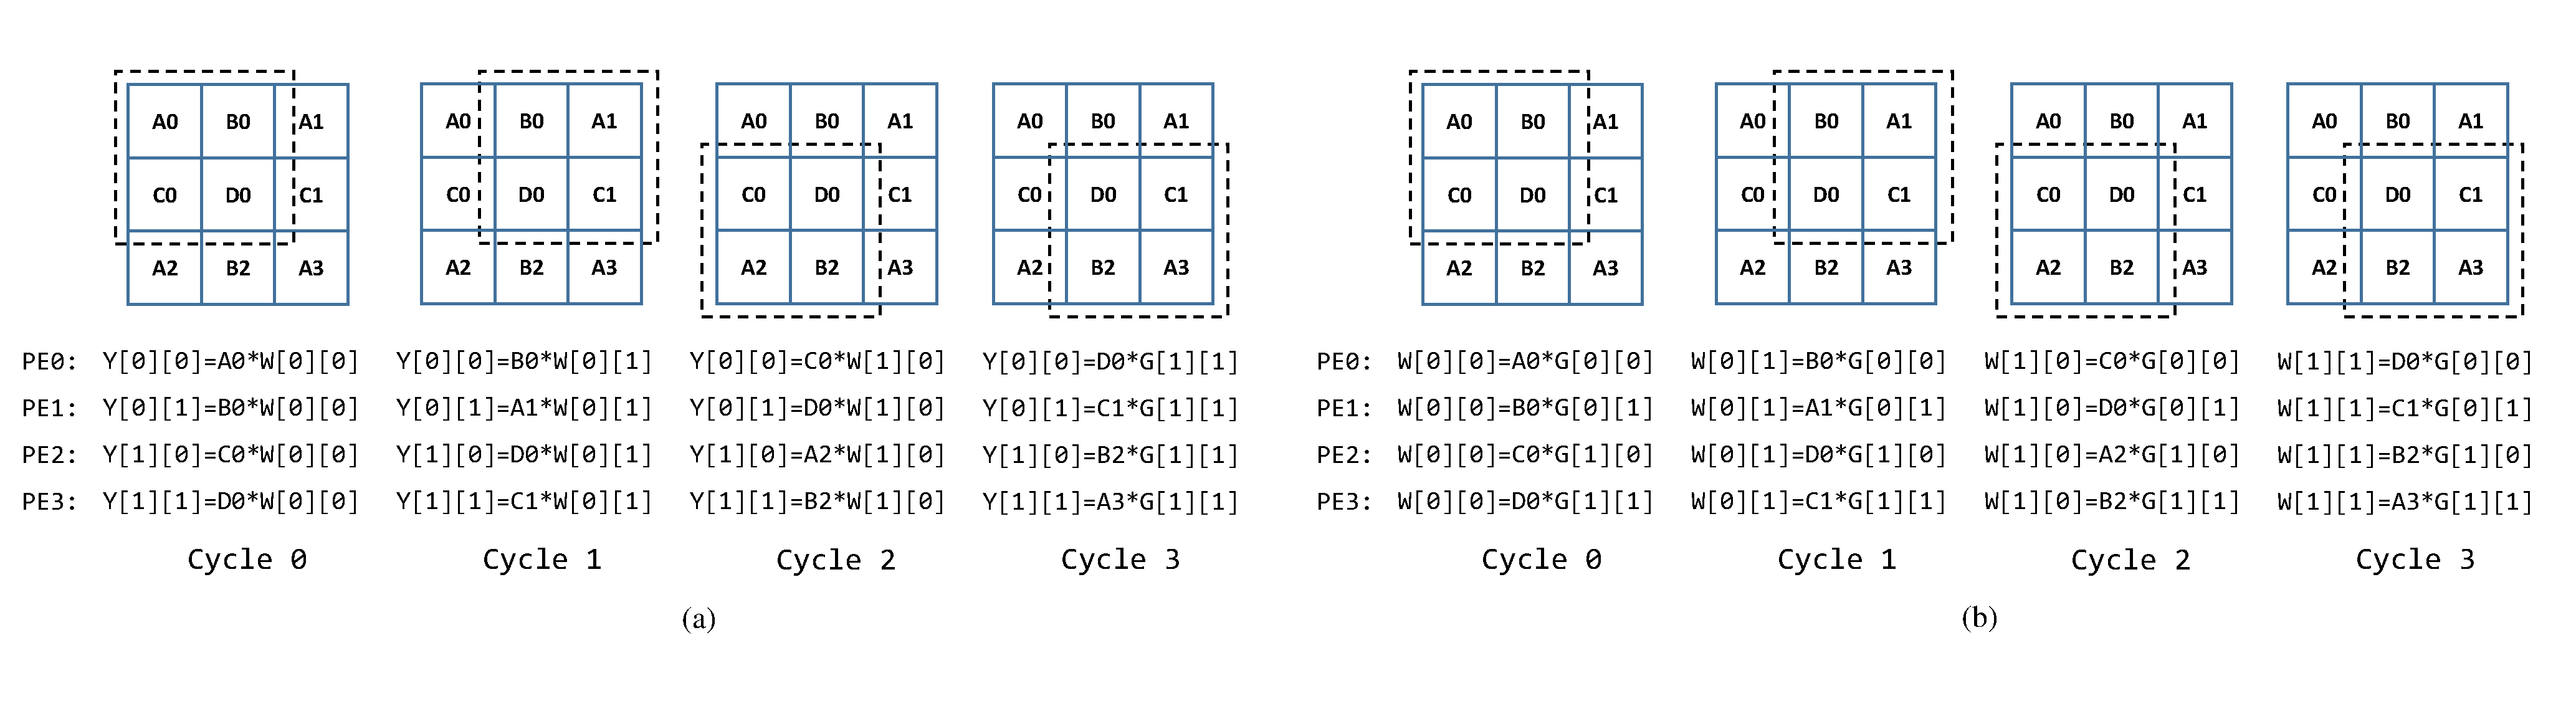
\includegraphics[width=2.0\columnwidth]{figures/mmap.pdf}
  \caption{Example of $2\times 2$ convolution on $3\times 3$ feature map with 4 PEs. The letter in each pixel denotes the PE it belongs to. The number denotes the address it stores in the buffer. The feature map needed for each cycle is marked with the dashed line box. (a) convolution in FF step. (b) convolution in WG step.}
  \label{fig:mmap}
\end{figure*}

So we choose to unroll batch and not implement layer pipeline. Each PE implements $b$ MAC units to process $b$ inputs in parallel. To reduce the channel level parallelism, we explore the possibility of unrolling feature map and convolution kernel dimension in CONV layers. We propose a configurable unroll method between these two dimension. 

For FF and NG steps, we let each $m$ PEs compute $m$ output pixels of a same feature map in parallel. To save on-chip buffer, we split the feature map to $m$ PEs and enables data sharing among them with multiplexers. An example of a $2\times 2$ convolution on a $3\times 3$ feature map with 4PEs are shown in Figure~\ref{fig:mmap}(a). In each cycle, all the PEs fetch the same convolution kernel, multiplies it with a pixel and locally accumulate the result. After 4 cycles, the convolution is done. Note that except for the first cycle, no PE fetches data from its own buffer, which is enabled by data sharing.

For WG step, we let each $m$ PEs fetches $m$ different convolution kernels (in this step is the feature map gradient) and accumulate the result for a same output pixel in parallel. This example is shown in Figure~\ref{fig:mmap}(b). The result are added together when data is written back to external memory. 

\subsection{Data Organization}
\begin{figure}[htb]
  \centering
  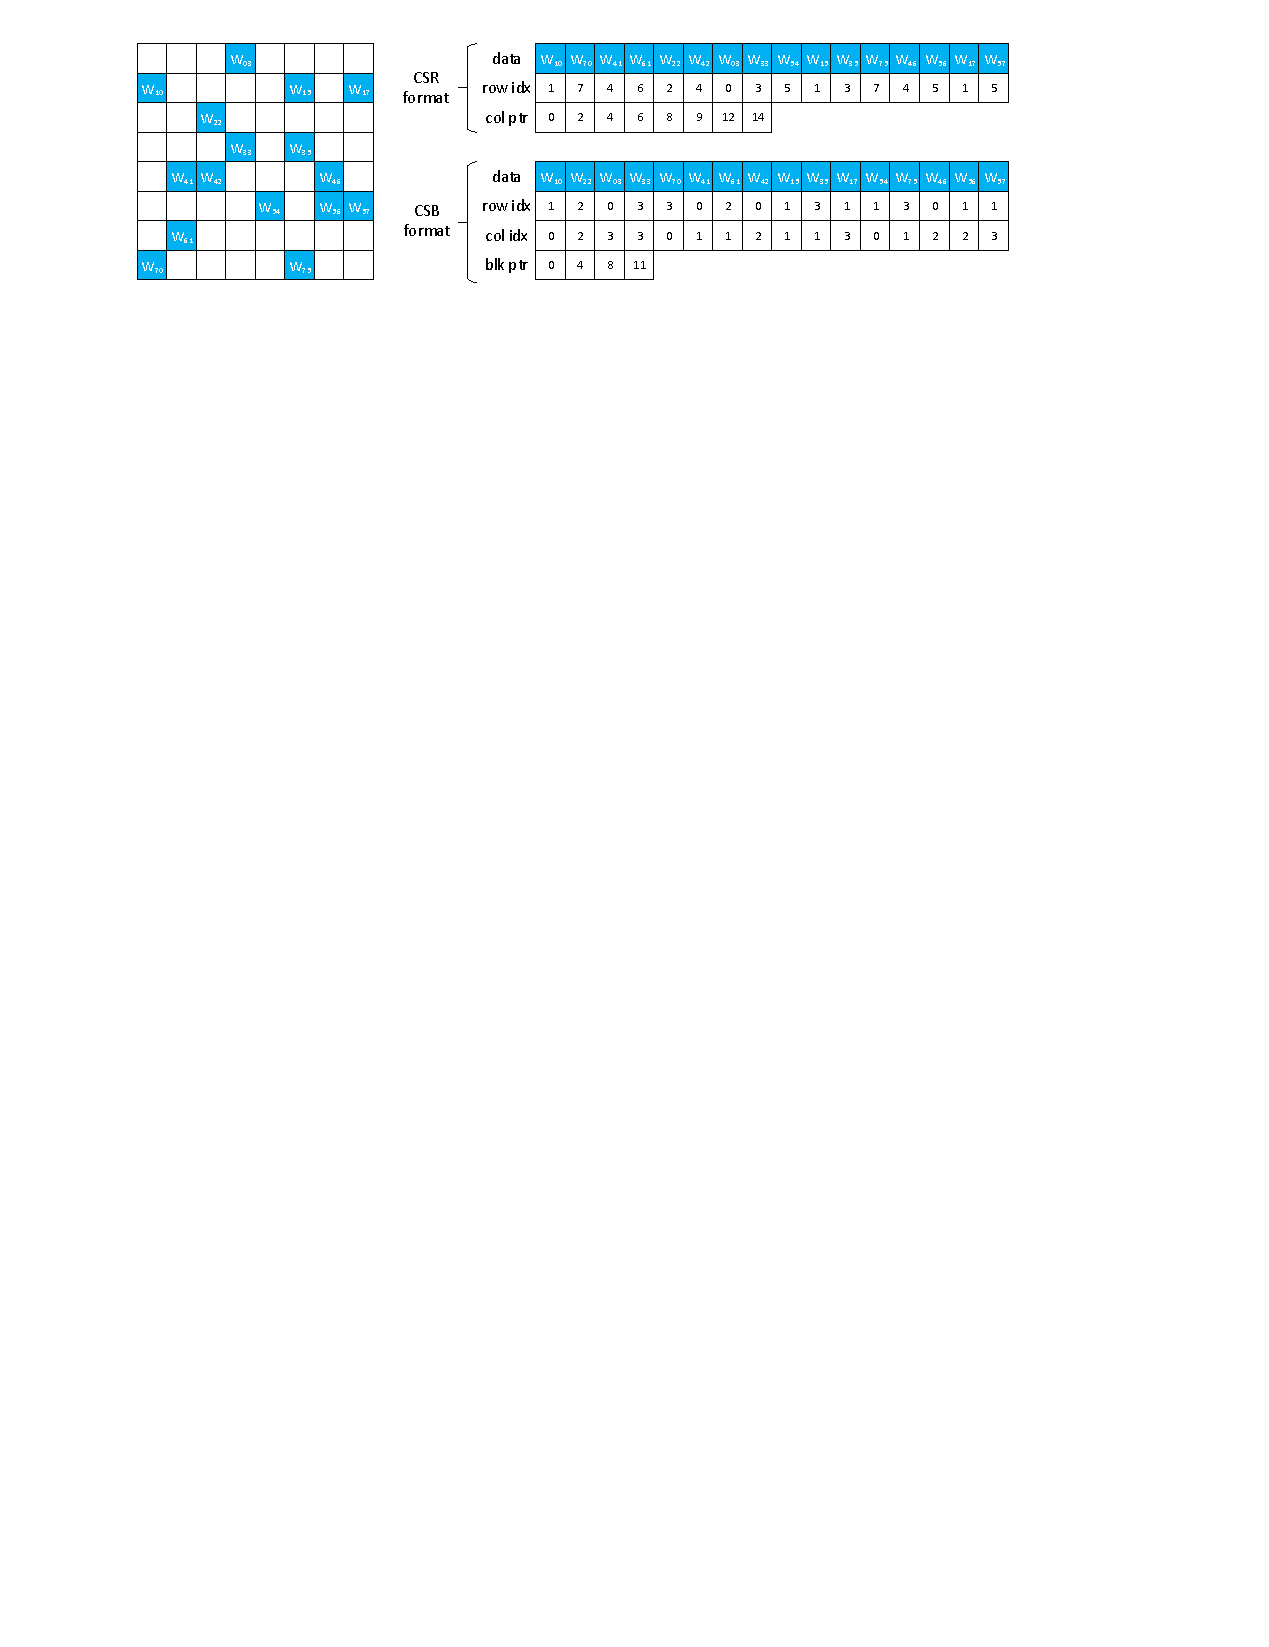
\includegraphics[width=1.0\columnwidth]{figures/csb.pdf}
  \caption{Example of different sparse matrix store formats for structured sparse convolution kernels. (a) Compressed Sparse Column(CSC) (b) Compressed Sparse Block(CSB)}
  \label{fig:csb}
\end{figure}

First, we use the compressed sparsed block (CSB) data format for the sparse weight storage. The sparse weight For fully connected layer, the inference phase and back propagation phase needs to access the parameter matrix in the original version and a transposed version. For convolutional layer, this is similar if we treat it as a 2-D matrix of 2-D convolution kernels. The commonly adopted CSC format, as shown in Figure~\ref{fig:csb}(a) stores data column by column, thus leads to the difficulty in row major access. So we adopt the CSB format~\cite{bulucc2009parallel} where the elements are encoded block by block. In this format, the access direction can be controlled by changing the access order of blocks. This format also fit with the hardware's block-wise process behavior as introduced in section~\ref{sec:hw_pe}. Since the transpose of a single block is achieved in PE level, we can access the sparse weights in both original and transposed format.

Second, we increase the access continuity of feature map by using a $(CHWC_mN)$ storage format. As introduced above, we process the channels in a block manner, and we always process the batch in parallel. So we store a batch of a same pixel continuously. Then, we store each $d$ channels of this pixel together.  $d$ is chosen the same as the corresponding convolution kernel block size of this layer. This requires that the output channel block size of one layer should be the same as the input channel block size of the next. So the memory access burst can reach $d*N*p$ where $p$ is the width to be processed each time, limited by on-chip buffer size and image width. 

\subsection{Scheduling Strategy}

\begin{figure*}[t]
  \centering
  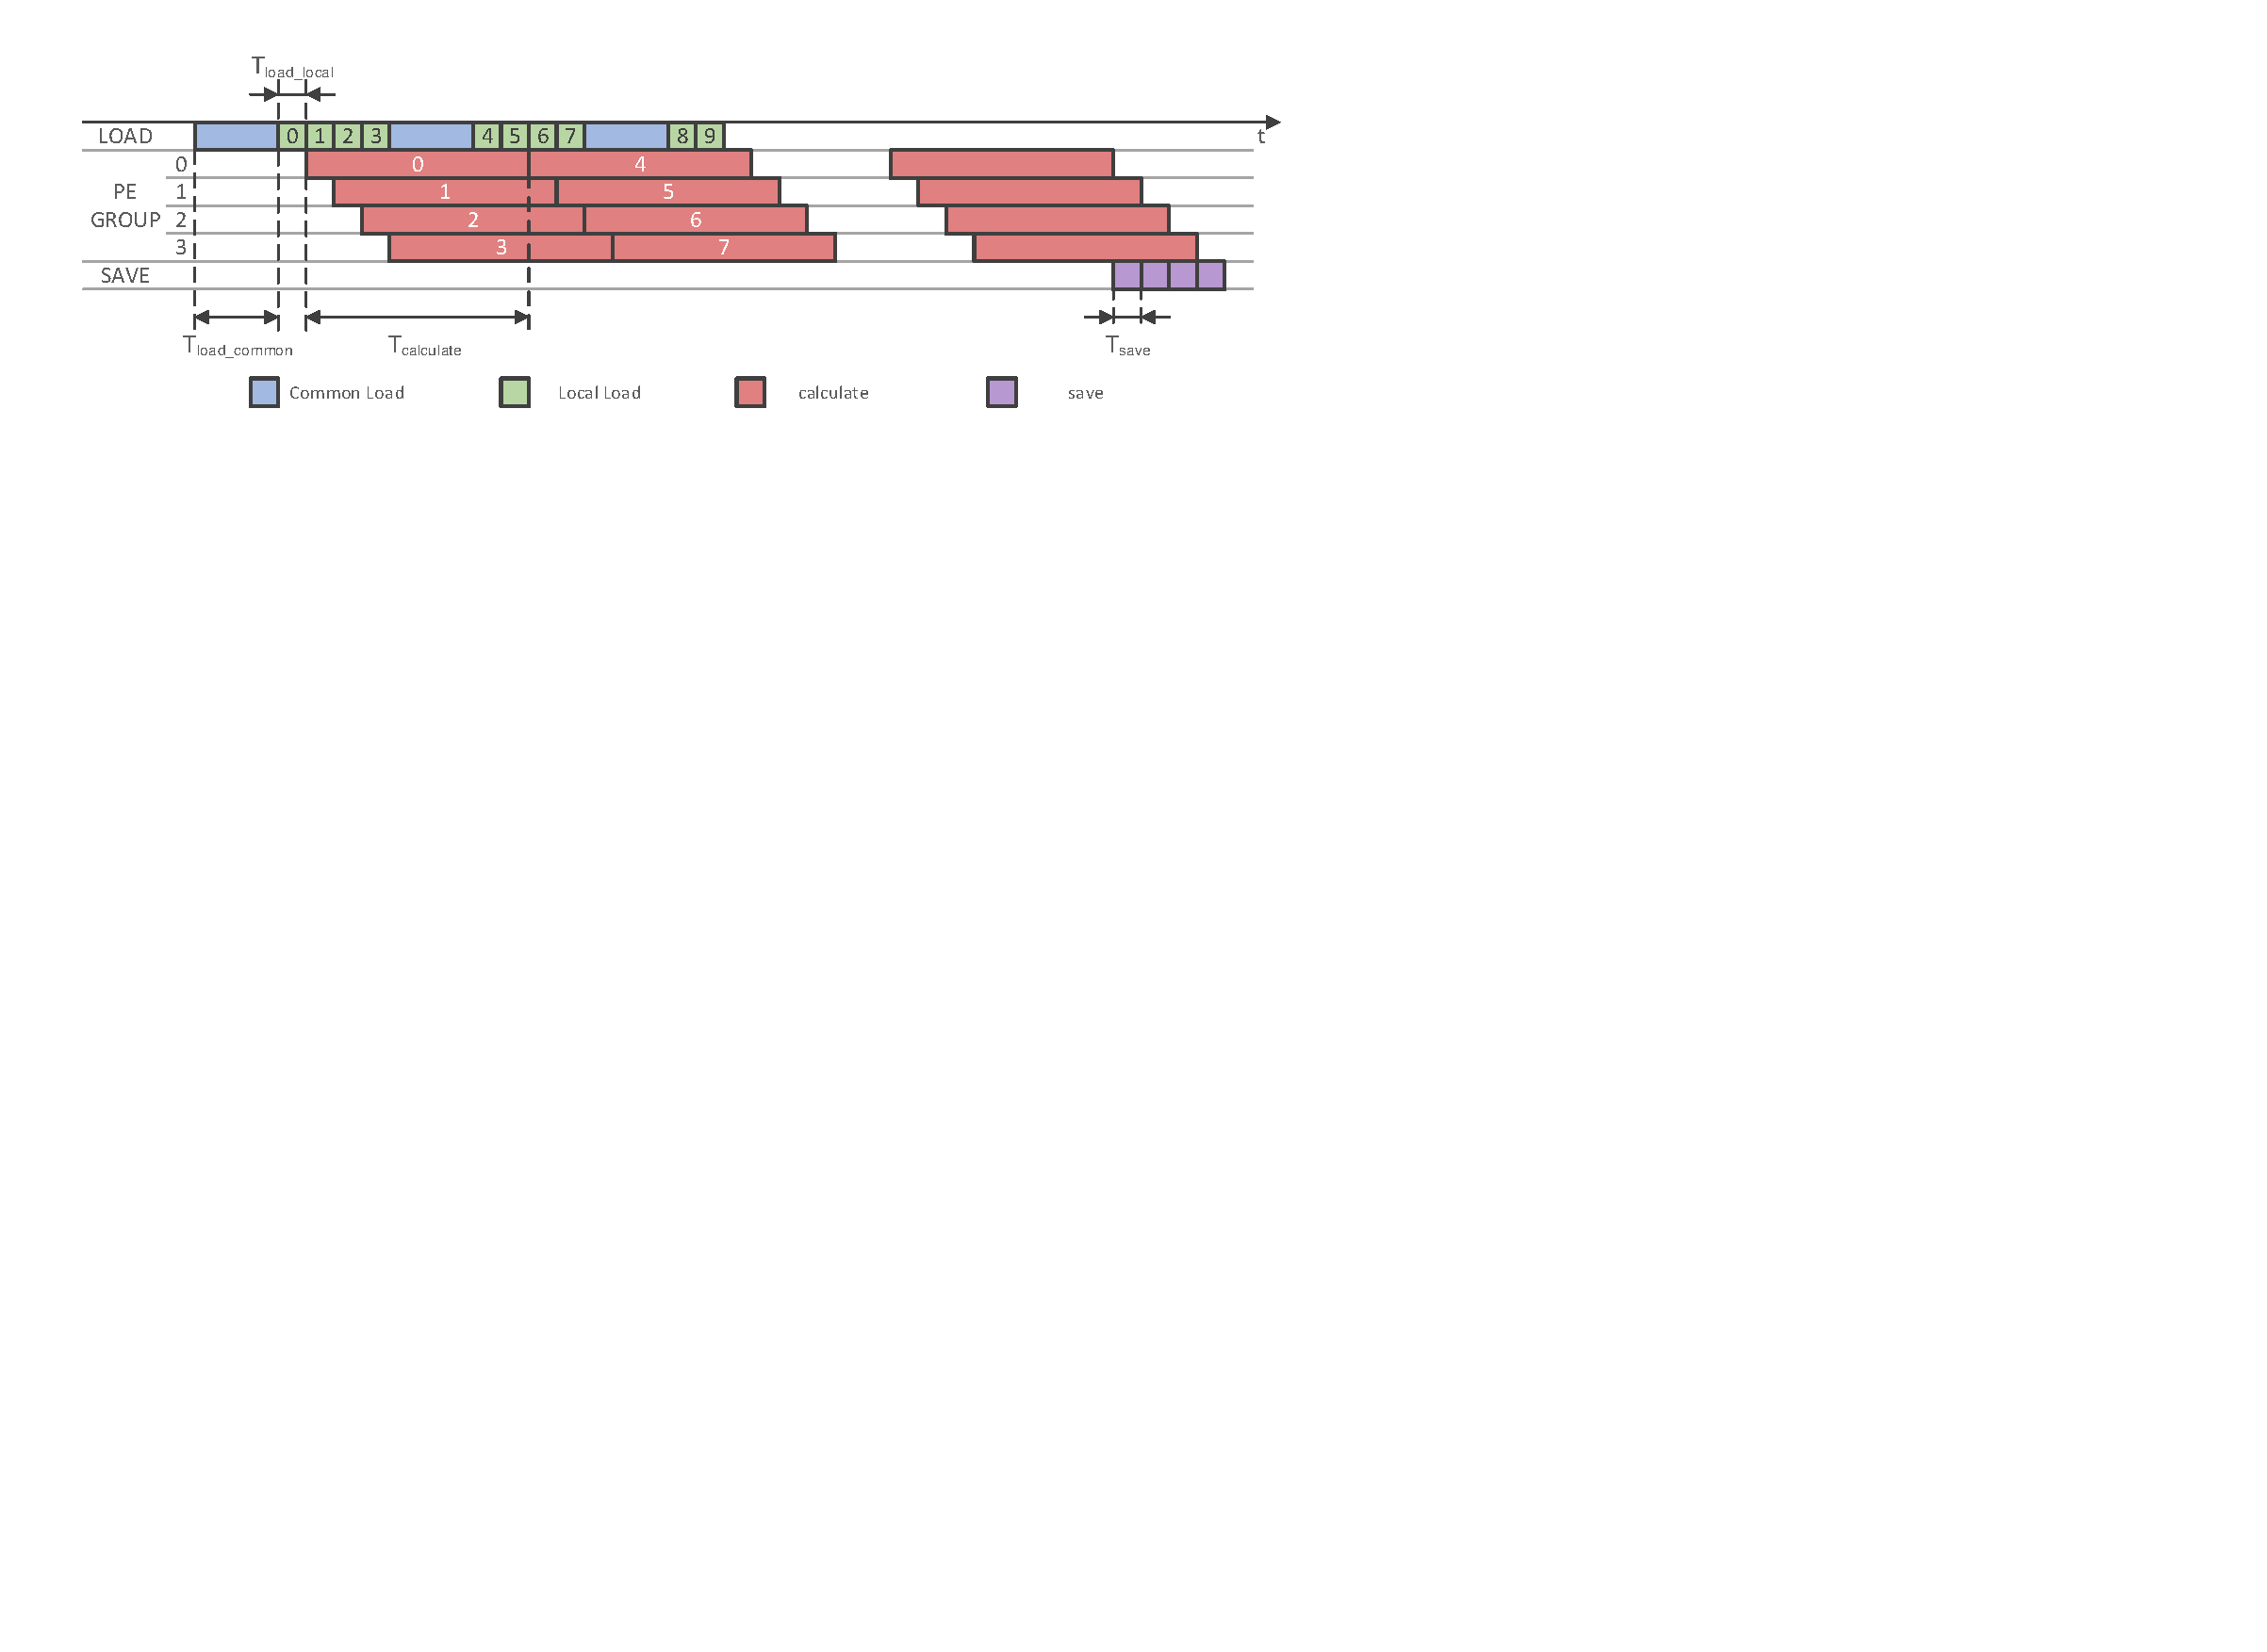
\includegraphics[width=1.8\columnwidth]{figures/schedule.pdf}
  \caption{Example scheduling time line. The number for load local and calculate denote the data dependency}
  \label{fig:sch}
\end{figure*}

As introduced above, each PE will process corresponding computations on a weight block each time. In our scheduling strategy, all the PEs will work with the same input channels/neurons, on different output channels/neurons. They first accumulate the result in ResBuf untill all the input channels are processed, then move on to the next set of output channels. For CONV layers, when all the (input, output) channel pairs are processed, the PEs will move on to the next part of feature map untill the whole feature map is processed. Mainly 4 types of operations are involved in the scheduling strategy.
\begin{itemize}
	\item {{\bf{Common Load}}: Load common data from external memory to all the PEs. In FF and WG steps, this is the common feature maps. In NG step, this is the common feature map gradient.}
    \item {{\bf{Local Load}}: Load local data to a PE or a group of PE. In FF and NG steps, this is the network weights and index. In WG step, this also includes weights buffer.}
    \item {{\bf{Calculation}}: Run a single or group of PE to process a weight block.}
    \item {{\bf{Save}}: Save the result of a single or group of PE to external memory.}
\end{itemize}
Load operation, each PE(PE group), and save operation can work in parallel. Figure~\ref{fig:sch}(a) shows an computation bounded time line example of a system with 4 PE groups. As long as $T_{calc}>T_{load\_common} + T_{load\_local}\times N_{pe}$, the system is computation bounded. Note that in real cases, $T_{calc}$ varies between different PEs and along time as the sparsity is random. $T_save$ can usually be ignored because it appears much less than load.   



\section{Experiment}\label{sec:experiment}
In section~\ref{sec:training}, we have shown the model accuracy and epoch consumption of the proposed hardware friendly training process. In this section, we show the hardware experimental results. A prototype design is implemented on a Xilinx XCKU115 chip with 2 on-board DDR4 SDRAM. In this system, feature map, neuron and their gradients are all of 8-bit and stored in DDR0. Network weights, each of which includes 8-bit MSB for computation and 24-bit LSB buffer, are stored in DDR1. Corresponding index for sparse representation are stored in DDR0 using \{y[3:0], x[3:0]\} format. This means the the maximum weights block size can be $16\times 16$. The system operates at 200MHz. Each $2\times 2$ PEs are grouped together for CONV layers.

\begin{table}[tb]
  \centering
  \caption{Prototype design resource utilization}
    \begin{tabular}{|c|c|c|c|c|}
    \hline
    Resource & LUT   & Reg   & Block RAM & DSP \\
    \hline
    Available & 663360 & 1326720 & 2160  & 5520 \\
    \hline
    Utilization & 193821 & 144594 & 1216   & 1024 \\
    \hline
    Ratio & 29\%  & 11\%  & 56\%  & 19\% \\
    \hline
    \end{tabular}
  \label{tab:util}
\end{table}

\subsection{Effect of Workload Imbalance}\label{sec:exp:imb}

Before introducing the hardware performance, we first analyze the theoretical performance loss brought by workload imbalance in Table~\ref{table:sparsity}. As introduced in section~\ref{sec:hw_unroll}, unroll parameters are limited by loop dimension variety and sparsity. As we cannot group the PEs for fully connected layers, we only compare on the convolutional layers. The normalized speed on the convolutional layers of each configuration is shown in Table~\ref{tab:hw_util}.

\begin{table}[tb]
  \centering
  \caption{Comparison of PE utilization with different group sizes on a network}
    \begin{tabular}{|c|c|r|r|r|r|r|}
    \hline
    \multirow{2}[4]{*}{Layer} & Feature & Workload & \multicolumn{3}{c|}{Utilization} \\
\cline{4-6}          & size & (MOP) & Single & 2x2 & Ideal\\
    \hline
    conv1 & $32\times 32$ & 3.54 & 80    & 88.5  & 100\\
    \hline
    conv2 & $16\times 16$ & 151 & 88.6  & 95.8  & 100\\
    \hline
    conv3\_1 & $8\times 8$   & 37.7 & 95.1  & 98.2  & 100\\
    \hline
    conv3\_2 & $8\times 8$   & 75.5 & 96.4  & 98.8  & 100\\
    \hline
    conv4\_1 & $4\times 4$   & 37.7 & 96.3  & 98.7  & 100\\
    \hline
    conv4\_2 & $4\times 4$   & 75.5 & 95.6  & 98.4  & 100\\
    \hline
    conv5\_1 & $2\times 2$   & 18.87 & 93.5  & 97.8  & 100\\
    \hline
    conv5\_2 & $2\times 2$   & 18.87 & 93.5  & 97.8  & 100\\
    \hline
    \multicolumn{3}{|c|}{Normalized Speed} & 1     & 1.050 & 1.078 \\
    \hline
    \end{tabular}
  \label{tab:hw_util}
\end{table}

\begin{figure}[tb]
  \centering
  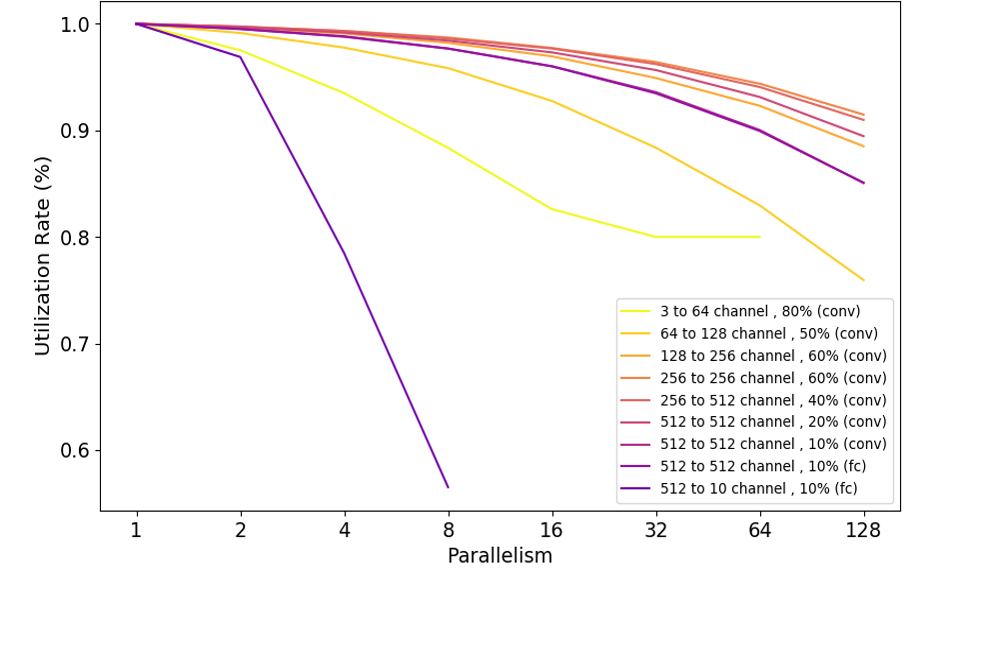
\includegraphics[width=1.0\columnwidth]{figures/util_real.png}
  \caption{Theoretical utilization ratio for each layer over the number of PEs.}
  \label{fig:util_real}
\end{figure}

Here, we see that using 32 PEs for this network will suffer from $7\%$ performance loss compared with the ideal case where no workload imbalance occurs. Group each 4 PEs together brings about $5\%$ performance increase. %Figure~\ref{fig:util_real} shows the utilization ratio of each layer over the number of PE(PE groups). The performance loss in the second layer contributes the most. Further increase the number of PEs will 


\subsection{Hardware Performance}
We simulate the performance of each layer in each training step with the DDR model and controller from Xilinx IP. Detailed running time and performance are shown in Table~\ref{tab:layerperformance}.

% Table generated by Excel2LaTeX from sheet 'Sheet4'
\begin{table*}[tb]
  \centering
  \footnotesize
  \caption{The performance of each layer. \textit{Comp.} indicates the complexity of each layer. \textit{Perf.} indicates the performance of running each layer on our hardware. \textit{Bound type} indicates the performance of each layer is bounded with bandwidth (B) or computation (C).}
% Table generated by Excel2LaTeX from sheet 'Sheet4'
\begin{tabular}{|c|c|c|c|c|c|c|c|c|c|c|c|c|c|}
\hline
      &       & \multicolumn{4}{c|}{Feed Forward (FF)}  & \multicolumn{4}{c|}{Neuron Gradient(NG)} & \multicolumn{4}{c|}{Neuron Gradient(NG)} \bigstrut\\
\cline{2-14}layer & Comp. & Time  & Perf. & bound & Utilize & Time  & Perf. & bound & Utilize & Time  & Perf. & bound & Utilize \bigstrut[t]\\
      & (GOP) & (us)  & (GOP/s) & type  & rate  & (us)  & (GOP/s) & type  & rate  & (us)  & (GOP/s) & type  & rate \bigstrut[b]\\
\hline
conv1 & 0.11  & 733   & 154.4  & B     & 27\%  & -     & -     & -     & -     & 4158  & 27.2  & B     & 5\% \bigstrut\\
\hline
conv2 & 1.21  & 1487  & 812.2  & C     & 95\%  & 1487  & 812.5  & C     & 95\%  & 2804  & 430.8  & B     & 50\% \bigstrut\\
\hline
conv3\_1 & 1.21  & 1696  & 712.4  & C     & 97\%  & 1694  & 713.0  & C     & 97\%  & 2477  & 487.7  & B     & 67\% \bigstrut\\
\hline
conv3\_2 & 2.42  & 2877  & 839.7  & C     & 98\%  & 2876  & 840.1  & C     & 98\%  & 4398  & 549.3  & B     & 64\% \bigstrut\\
\hline
conv4\_1 & 1.21  & 1217  & 992.3  & C     & 97\%  & 1217  & 992.9  & C     & 97\%  & 2686  & 449.8  & B     & 44\% \bigstrut\\
\hline
conv4\_2 & 2.42  & 1457  & 1658.4  & C     & 97\%  & 1456  & 1659.2  & C     & 97\%  & 3933  & 614.2  & B     & 36\% \bigstrut\\
\hline
conv5\_1 & 0.60  & 366   & 1651.7  & B     & 32\%  & 358   & 1687.7  & B     & 33\%  & 915   & 659.8  & B     & 13\% \bigstrut\\
\hline
conv5\_2 & 0.60  & 365   & 1652.7  & B     & 32\%  & 358   & 1688.7  & B     & 33\%  & 915   & 660.0  & B     & 13\% \bigstrut\\
\hline
dense6 & 0.02  & 329   & 51.0  & B     & 1\%   & 328   & 51.1  & B     & 1\%   & 717   & 23.4  & B     & 0.5\% \bigstrut\\
\hline
dense7 & 0.02  & 329   & 51.0  & B     & 1\%   & 328   & 51.1  & B     & 1\%   & 717   & 23.4  & B     & 0.5\% \bigstrut\\
\hline
dense8 & 0.003  & 75    & 4.4   & B     & 0.1\% & 74    & 4.4   & B     & 0.1\% & 272   & 1.2   & B     & 0.02\% \bigstrut\\
\hline
total & 9.81  & 10931  & 897.5  & -     & -     & 10988  & 892.8  & -     & -     & 23993  & 408.9  & -     & - \bigstrut\\
\hline
\end{tabular}%
  \label{tab:layerperformance}%
\end{table*}%

% Table generated by Excel2LaTeX from sheet 'Sheet4'
\begin{table*}[tb]
  \centering
  \caption{Performance and energy efficiency comparison with GPU. }
    \begin{tabular}{|c|c|c|c|c|c|c|c|}
    \hline
          & Data Format & Forward time & Backward time & Total time & Performance & Power & Power efficiency \bigstrut[t]\\
          & data+gradiant & (us)  & (us)  & (us)  & (GOP/s) & (W)   & (GOP/s/W) \bigstrut[b]\\
    \hline
    GPU   & float + float & 7795  & 15700  & 23495  & 1252.7  & 150   & 8.4  \bigstrut\\
    \hline
    FPGA  & 8bit + 24bit & 10931  & 34981  & 45912  & 641.1  & 29    & 22.1  \bigstrut\\
    \hline
    \end{tabular}%
  \label{tab:exp_comp}%
\end{table*}%

The peak performance of the hardware is $250MHz \times 1024DSP \times 2 = 500GOP/s$. For FF and NG steps, the proposed hardware achieves 900GOP/s overall performance which achieves at least $1.8\times$ speedup over a dense accelerator with the same peak performance. From the bound type column, we see that most of the CONV layers with heavy workload are computation bounded. This shows that the proposed accelerator can handle large network well.

A performance and energy efficiency comparison is shown in Table~\ref{tab:exp_comp}. The GPU used for comparison is GTX Titan X GM200. Alough GPU achieves about 2x speed compared with FPGA, the FPGA part only consumes 1/5 power compared with GPU and achieves 3x energy efficiency.

Besides that, those layers which are bandwidth bounded gives insights to hardware design methods. The first layer suffers from the bandwidth problem because the channel number for this layer is small. We only cut $3\times 8$ block for this layer. A small block size increases the ratio between the necessary feature maps and the necessary convolution kernels. Compared with the workload imbalance result in \ref{sec:exp:imb}, we see that small layers suffer more on bandwidth rather than workload imbalance. Besides reducing the number PEs, increase the buffer size in PEs can help further explore the data locality of 2-d convolution and improves performance. 

The last few layers also suffers greatly from a limited bandwidth. On the one hand, FC layers and convolution layers with small feature maps are of high bandwidth cost for network parameters. On the other hand, split the parameters into small blocks decreases the memory access efficiency. Increase the the 

When upgrading the weights of each layer, the weight buffer consumes more bandwidth and causes the performance loss. Reduce the weight buffer size should also be a future research topic. 







\section{Related Work}\label{sec:related_work}
In this section, we will introduce related work on software and hardware respectively. For software, we will focus on neural network training with fixed-point data and pruned parameters. For hardware, as few previous work targets at training acceleration, we will focus on inference accelerators.

\subsection{Training with Fixed Point Data}
Usually, neural network models are trained and used with 32-bit floating point data on GPU or CPU. An effective way for neural network acceleration is to use fewer bits for data in NN models to reduce memory cost and simplify each of the operation.

For inference, many work~\cite{han2016eie,qiu2016going} show that 8-bit or even fewer bits can be used to achieve significant acceleration on customized hardware architectures with negligible accuracy loss. Courbariaux et al.\cite{NIPS2016_6573} demonstrate how to train a binary NN model which brings relatively small accuracy loss on the CIFAR-10 dataset. Tang et al.~\cite{Tang2017HowTT} focus on how to enable better training of a BNN(binarized NN) on larger datasets using strategies such as small learning rate, bipolar regularization, etc.

Some work also studies how to perform the training process with fixed-point gradients~\cite{NIPS2016_6573,Hubara2016Quantitized,Zhou2016DoReFa}, in these work, not only the weights and the activations, the gradients in the training process are also quantized. Zhou et al.~\cite{Zhou2016DoReFa} quantize the weights to 1 bit, activations to 2 bit, and the gradients of activations to 6 bit. Their quantization method is to uniformly quantize each blob between $[-\mbox{absmax}, \mbox{absmax}]$, and a floating-point $\mbox{absmax}$ value must be stored for each blob. To do quantization, they need global information of each blob (calculate the floating-point number of each blob). Although the bit-width of data blobs is low in these work, they all require storing floating-point scale factors with floating-point operations for multiplication and gradient distribution statistics. {\bf{Floating point operations are still of high cost while total fixed-point based training process still needs research.}}


\subsection{Neural Network Pruning}
Pruning is an efficient method to reduce both the model size and the number of operations by removing insignificant parameters, which helps achieve neural network acceleration. Han et al.~\cite{han2015learning} introduced a direct method by iteratively pruning parameters below the threshold and fine-tuning. Such element-wise pruning (0-dimension pruning) is powerful for compression and reduces storage 9x-13x. However, the irregularity of the pruned model brings a challenge for executing the network efficiently on hardware. Some researches focus on exploring group-wise sparsity (1-dimension or 2-dimension pruning)\cite{lebedev2016fast,zhou2016less,wen2016learning} of the convolution filters. Recently, pruning filters (3-dimension pruning)\cite{molchanov2016pruning,li2016pruning} is proposed to reduce model size while totally keeping the model regularity. As suggested by Mao et al.\cite{mao2017exploring}, 0 to 2-dimension pruning does negligible harm to the network accuracy while 3-dimension pruning incurs great accuracy loss. In this work, we choose 2-dimension pruning which keeps acceptable model accuracy and relatively good regularity.

\subsection{Dense CNN Inference Accelerator}\label{sec:rw_dense}
Many hardware designs have been proposed to accelerate dense CNN inference. As suggested by~\cite{ma2017optimizing}, for a single layer, a CNN inference accelerator design involves three aspects: loop unrolling, loop tiling, and loop interchange. Loop unrolling strategy decides the parallelism or the peak performance of the hardware. \cite{zhang2015optimizing, du2015shidiannao, qiu2016going} explore different unroll dimensions and hardware designs respectively. Loop tiling and loop interchange strategy decide how the computation of this layer is scheduled. When the data needs to be loaded from external memory, a good loop tiling and loop interchange strategy helps minimize bandwidth requirement and maximize the utilization of hardware computation power. For CNN training, the back propagation also consists of nested loops. Thus the same design methods can be applied.

For a whole network, a strategy for one layer is usually hard to be fit into the other layers. Loop tiling and loop interchange can be controlled by software while loop unrolling strategy is hard to change at run-time. One solution is to implement different hardware for different layers as a pipeline~\cite{Li2016High}. This method is usually resource consuming and lacks flexibility for different networks. Another way is to use a flexible structure for computation unit array. \cite{chen2016eyeriss} proposes a run-time configurable PE array structure. In this design, all the PEs are configured with certain id and multiple buses are used to adapt to different data transfer behavior under different configurations. However, this kind of bus based structure cannot be efficiently implemented on FPGA.

For CNN training, as suggested by section~\ref{sec:preliminary}, the loops in back propagation phase is similar to that in inference phase. But the loop dimension varies greatly between the feed forward and back propagation phases. For example, if a convolutional layer does $3\times 3$ convolution on $224\times 224$ feature maps with 1 padding, computing the gradient of these convolution kernels needs $224\times 224$ convolutions on $224\times 224$ feature maps with 1 padding. {\bf{This causes great variety in convolution kernels and convolution result sizes and thus limits the loop unroll design.}} 

\subsection{Sparse CNN Inference Accelerator}\label{sec:rw_sparse}
With the research progress in neural network model pruning, more and more work focus on accelerating sparse CNN inference. One kind of work focus on utilizing the sparsity of network parameters~\cite{han2017ese,zhang2016cambricon}, which is denoted by $S\times D=D$ type. \cite{albericio2016cnvlutin} utilizes the data sparsity brought by ReLU function, which is denoted by $D\times S=D$. \cite{han2016eie} utilizes both the sparsity of data and parameters. For CNN training with sparse parameters, a new type of sparse computation, $D\times D=S$ is needed. When calculating the gradient of network parameters, the operators are activation of one layer and the gradient of the activation of the next layer, which can both be dense. But we do not need to compute the gradient of the pruned parameters. So the result is sparse. In this work, we propose an architecture to support both $S\times D=D$ and $D\times D=S$ computation.



\section{Conclusion}\label{sec:conclusion}

In this paper, we accelerate neural network training with both software optimization and hardware design. We propose a hardware friendly training process where the fine-tune stage are totally based on fixed-point data computation and using a 2 dimension pruning method to produce regular model sparsity. Specialized processing units are designed to utilize model sparsity in both the inference and back propagation phases for acceleration. A hardware accelerator is designed to adapt to the great loop dimension variety between CNN inference phase and back propagation phase and cover bandwidth cost with certain data arrangement and schedule strategy. Proposed hardware achieves 641GOP/s equivalent performance and 3x better energy efficiency compared with GPU. 

%%%%%%% -- PAPER CONTENT ENDS -- %%%%%%%%

%%%%%%%%% -- BIB STYLE AND FILE -- %%%%%%%%
\bibliographystyle{ieeetr}
\bibliography{ref}
%%%%%%%%%%%%%%%%%%%%%%%%%%%%%%%%%%%%

\end{document}